\documentclass[12pt,a4paper, fleqn]{report}

\usepackage[utf8]{inputenc}
\usepackage[french]{babel}
\usepackage{tikz}
\usepackage[T1]{fontenc}
\usepackage{amsmath}																				% les maths
\usepackage{amsfonts}
\usepackage{amssymb}
\usepackage{fourier}																					% symboles intégral propre
\usepackage{graphicx}
\usepackage[left=2cm,right=2cm,top=2cm,bottom=2cm]{geometry}	% les marges
\usepackage{multicol}																					% pour écrire sur plusieurs colones
\usepackage[thinspace,thinqspace,amssymb]{SIunits}							% écriture des nombres et unités
\usepackage{setspace}																				% set space between lines
\usepackage{array}																						% stretch array lines
\usepackage[hyphens]{url}
\usepackage[breaklinks]{hyperref}															% clickable links
%\usepackage[hyphenbreaks]{breakurl}														% for long urls
\usepackage{chemfig}																					% pour les formules chimiques
\usepackage{pdflscape}

\hypersetup{
    colorlinks=true,
    linkcolor=red_f,
    citecolor=bleu_f,
    filecolor=green_f,
    urlcolor=bleu_f
}

\usepackage{xcolor}																			% colors
\usepackage[framemethod=tikz]{mdframed}									% fancy environments

%%%%%%%%%% graphic charter

\renewcommand{\familydefault}{\sfdefault}												% sans serif font

%%%%% HEADER
%\pagestyle{fancy}
%\lhead{\textcolor{gray_f}{Physique-Chimie\\R. METZDORFF}}
%\chead{\textcolor{gray_f}{Lycée Suzanne Valadon}}
%\rhead{\textcolor{gray_f}{2020-2021}}
%\renewcommand{\headrulewidth}{0.4pt}
%\let\HeadRule\headrule
%\renewcommand\headrule{\color{gray_f}\HeadRule}

%%%%% COLORS
\definecolor{gray_f}{RGB}{68,84,106}
\definecolor{gray_c}{RGB}{214,220,229}
\definecolor{gray_cc}{RGB}{245,245,245}
\definecolor{bleu_f}{RGB}{91,155,213}
\definecolor{bleu_c}{RGB}{222,235,247}
\definecolor{red_f}{RGB}{204,0,0}
\definecolor{red_c}{RGB}{245,204,204}
\definecolor{orange_f}{RGB}{237,125,49}
\definecolor{orange_c}{RGB}{251,229,214}
\definecolor{green_f}{RGB}{112,173,71}
\definecolor{green_c}{RGB}{226,240,217}
\definecolor{yellow_f}{RGB}{255,192,0}
\definecolor{yellow_c}{RGB}{255,242,204}
\definecolor{code_keyword}{RGB}{23,23,139}										% colors for pyhton code
\definecolor{code_comment}{RGB}{50,137,21}
\definecolor{code_string}{RGB}{139,139,25}
\definecolor{red_unilim}{RGB}{166,41,41}
\definecolor{gray_unilim}{RGB}{78,87,94}
\definecolor{orange_unilim}{RGB}{209,98,40}

%%%%% NEW ENVIRONMENTS

%%% header
\mdfdefinestyle{s_head}{%
	linecolor=red_unilim!,
	outerlinewidth=3pt,%
	frametitlerule=false,
	topline=false,
	bottomline=false,
	rightline=false,
	leftline=false,
	backgroundcolor=red_unilim,
	innertopmargin=8pt,
	roundcorner=0pt,
	nobreak=true,
	fontcolor=white
}
\newmdenv[style=s_head]{header_env}
\newenvironment{header}
{%\stepcounter{exa}%
	\addcontentsline{ldf}{figure}{0}%
	\begin{header_env}\qquad\Large\bf}
	{\end{header_env}}

%%%%% New command

\newcommand{\app}{\colorbox{bleu_c}{\textcolor{bleu_f}{APP}}}
\newcommand{\rea}{\colorbox{yellow_c}{\textcolor{yellow_f}{REA}}}
\newcommand{\anarai}{\colorbox{green_c}{\textcolor{green_f}{ANA-RAI}}}
\newcommand{\val}{\colorbox{orange_c}{\textcolor{orange_f}{VAL}}}
\newcommand{\com}{\colorbox{red_c}{\textcolor{red_f}{COM}}}
\newcommand{\auto}{\colorbox{white}{\textcolor{black}{AUTO}}}
\newcommand{\rco}{\colorbox{gray_c}{\textcolor{gray_f}{RCO}}}
\newcommand{\seconde}{2\textsuperscript{nde}}

\bibliographystyle{custom-bib/thesis}
\usepackage{bibentry}
\usepackage{pdfpages}

\title{L'expérience de Benjamin Franklin... Et Rayleigh, Pockels, Devaux, et Langmuir}
\author{Rémi Metzdorff}
\date{\today}

\onehalfspacing

\begin{document}

%\maketitle

\begin{header}
\begin{minipage}{0.55\textwidth}
Rapport de stage (S3 -- S4)
\end{minipage}
\begin{minipage}{0.38\textwidth}
\href{https://www.unilim.fr/}{
\includegraphics[scale=1]{logo.png}}
\end{minipage}
\end{header}

\vspace{30pt}
\begin{spacing}{1.2}
{\bf
\begin{Large}
\noindent
\textcolor{gray_unilim}{INSPE Académie de Limoges}
\end{Large}

\begin{large}
\noindent
\textcolor{gray_unilim}{Métiers de l'enseignement, de l'éducation et de la formation}

\noindent
\textcolor{gray_unilim}{Master MEEF Second degré}

\noindent
\textcolor{gray_unilim}{Professeur de Physique et de Chimie}

\noindent
\textcolor{gray_unilim}{Accompagnement à la mise en situation professionnelle}

\end{large}
}

\vspace{20pt}

\noindent
\textcolor{gray_unilim}{2020--2021}

\vspace{40pt}
\begin{large}
\bf
\noindent
\textcolor{gray_unilim}{Analyse d'une séance autour de la mesure de la taille d'une molécule d'huile d'après l'expérience de Franklin}

\vspace{150pt}
\noindent
\textcolor{gray_unilim}{Rémi Metzdorff}

\noindent
\textcolor{gray_unilim}{Lycée Suzanne Valadon}
\end{large}
\end{spacing}

\vfill

\hfill

\includegraphics[scale=1]{logo_bottom.png}

\thispagestyle{empty}

\newpage

\tableofcontents
\newpage

\chapter{Analyse a priori de la séance}

\section*{Introduction}
\addcontentsline{toc}{section}{Introduction}

Ce chapitre présente la préparation d'une séance autour de l'expérience historique de Benjamin Franklin et de son interprétation par lord Rayleigh en vue de déterminer la taille d'une molécule.
Elle est prévue pour des élèves de seconde en demie-classe sur un créneau de TP d'une heure et vingt cinq minutes.

Pour cette année de stage, je suis affecté au lycée Suzanne Valadon à Limoges.\footnote{Lycée d'enseignement général et technologique Suzanne Valadon

39, rue François Perrin -- 87000 Limoges.

Téléphone : 05 55 45 56 00

E mail : ce.0870019y@ac-limoges.fr

Site internet : \href{http://www.lyc-valadon.ac-limoges.fr/}{http://www.lyc-valadon.ac-limoges.fr/}.}
Avoir avoir présenté l'organisation du lycée et ma situation en tant qu'enseignant stagiaire, c'est l'organisation de la séance qui sera détaillée.

\section{Le lycée Suzanne Valadon}

\subsection{Formations proposées}

Le lycée Suzanne Valadon est un établissement qui propose plusieurs formations.
C'est un lycée d'enseignement :
\begin{itemize}
\item[•] général : \hfill \textbf{354 élèves}
\begin{itemize}
\item 6 classes de secondes ;
\item 3 classes de premières ;
\item 3 classes de terminales.
\end{itemize}
\item[•] technologique (sciences et technologies de la santé et du social ou ST2S et sciences et technologies du management et de la gestion ou STMG) : \hfill \textbf{379 élèves}
\begin{itemize}
\item 4 classes premières ST2S et 2 classes de premières STMG ;
\item 4 classes terminales ST2S et 3 classes de terminales STMG.
\end{itemize}
\item[•] professionnel (accompagnement, soins et services à la personne ou ASSP) : \hfill \textbf{162 élèves}
\begin{itemize}
\item 3 classes de secondes ;
\item 3 classes de premières ;
\item 3 classes de terminales.
\end{itemize}
\end{itemize}

La filière générale scientifique est récente dans l'établissement puisque l'ouverture de la première scientifique remonte seulement à la rentrée de septembre 2016.
Suite à la réforme du lycée, l'établissement a pu maintenir la spécialité physique chimie et propose les enseignements de spécialité suivants depuis 2019 : 
\begin{itemize}
\item[•] arts -- arts plastiques ;
\item[•] arts -- danse ;
\item[•] histoire géographie, géopolitique et sciences politiques ;
\item[•] humanités, littérature et philosophie ;
\item[•] mathématiques ;
\item[•] physique chimie ;
\item[•] sciences économiques et sociales ;
\item[•] sciences de la vie et de la terre.
\end{itemize}

L'établissement propose également plusieurs formations post-bac :
\begin{itemize}
\item[•] 6 brevets de technicien supérieur ou BTS : \hfill \textbf{408 étudiants}
\begin{itemize}
\item gestion de la PME PMI ;
\item support à l'action managériale ;
\item comptabilité et gestion ;
\item management commercial opérationnel ;
\item services informatiques aux organisations ;
\item économie sociale et familiale.
\end{itemize}
\item[•] 1 diplôme de technicien supérieur en imagerie médicale et radiologie thérapeutique ou DTS IMRT ; \hfill \textbf{52 étudiants}
\item[•] 2 classes préparatoires au diplôme de comptabilité de gestion ou DCG et diplôme supérieur de comptabilité et de gestion ou DSCG ; \hfill \textbf{108 étudiants}
\item[•] 1 diplôme d'état conseiller en économie sociale et familiale ou DCESF. \hfill \textbf{24 étudiants}
\end{itemize}

Enfin, l'établissement héberge le micro-lycée Utrillo : \hfill \textbf{14 élèves}
\begin{itemize}
\item[•] 1 classe de premières ;
\item[•] 1 classe de terminales.
\end{itemize}

Il s'agit donc d'un établissement de taille assez conséquente puisqu'il rassemble environ 1\,500 élèves et étudiants.

\subsection{Résultats}

Les résultats aux baccalauréats généraux, technologiques et professionnels sur les dix dernières années sont présentés en annexe (Annexe~\ref{ann:resultats}).

\subsection{Organisation du lycée}

Le fonctionnement du lycée est assuré par l'ensemble de son personnel, soit près de 500 personnes, organisé autour de Madame la Proviseur Nadège Vergnaud et Monsieur le Proviseur-Adjoint Nicolas Chaume (Fig~\ref{fig:organigramme}, Annexe~\ref{ann:organigramme}).
Chacun a un rôle et des responsabilités bien définis \cite{Jourdan2016} :
\begin{itemize}
\item[•] la Proviseur est le représentant de l'état au sein de l'établissement et c'est elle qui représente l'établissement.
Elle est la représentante juridique.
Ses missions sont multiples : organisation, gestion, contrôle, etc.
\item[•] le Proviseur-Adjoint est le principal conseiller du chef d'établissement.
Son rôle est particulièrement important dans l'organisation quotidienne de la vie de l'établissement.
C'est notamment lui qui est en charge de l'organisation des emplois du temps.
\item[•] la gestionnaire est en charge du budget de l'établissement.
Elle est en charge de la gestion des personnels mais aussi des équipements du lycée.
\item[•] les conseillers principaux d'éducation (CPE) sont en charge du suivi et de l'accompagnement des élèves, notamment en gérant les absences et retards, et prennent part à la vie lycéenne.
Ils gèrent les assistants d'éducation (AED) qui s'assurent du bon déroulement de la vie scolaire.
\item[•] le pôle de soutien regroupe l'ensemble des personnels en charge notamment de l'accompagnement des élèves en difficulté.
Par exemple, les accompagnants des élèves en situations de handicap aident ces élèves et favorisent leur autonomie.
\item[•] le personnel technique et ouvriers de services (TOS) regroupe environ trente personnes en charge de l'entretien des infrastructures de l'établissement et du fonctionnement du restaurant scolaire.
\item[•] finalement les enseignants accompagnent les élèves dans leurs apprentissages.
L'établissement compte 137 enseignants.
\end{itemize}

Le lycée Suzanne Valadon a aussi la particularité d'héberger le pôle sanitaire et social du Greta du Limousin (\href{https://greta-du-limousin.fr/tagged/accueil}{https://greta-du-limousin.fr/tagged/accueil}).
Les groupements d'établissements (Greta) sont les structures de l'éducation nationale qui organisent des formations pour adultes dans de nombreux domaines professionnels. 

\subsection{Situation en tant que stagiaire}

Cette année, je suis donc stagiaire en responsabilité pour la discipline sciences physiques et chimiques au lycée Suzanne Valadon de Limoges.
Je m'occupe de l'enseignement de physique-chimie pour deux classes de secondes (\seconde1 et \seconde2) pour un total de 69 élèves (34 et 35).
Les cours en classe entière se font en séance d'une heure (une heure toutes les semaines et une heure en quinzaine, c'est-à-dire une semaine sur deux).
Chaque classe est divisée en deux groupes pour les séances de travaux pratiques d'une heure et demie.
J'assure donc un service de neuf heures réparties sur les trois premiers jours de la semaine (Annexe~\ref{ann:edt}).

Les élèves ont des profils variés et souhaitent s'orienter vers différentes filières :
\begin{itemize}
\item[•] générale : 23 élèves soit environ \unit{33}{\%} dont 11 élèves soit \unit{16}{\%} souhaitent poursuivre avec la spécialité physique-chimie ;
\item[•] ST2S : 11 élèves soit environ \unit{16}{\%} ;
\item[•] STMG : 10 élèves soit environ \unit{14}{\%} ;
\item[•] STD2A : 3 élèves soit environ \unit{4}{\%} ;
\item[•] technologique : 2 élèves soit environ \unit{3}{\%} ;
\item[•] orientation non déterminée en fin de premier trimestre : 20 élèves soit environ \unit{29}{\%}.
\end{itemize}

\section{Présentation de la séance}

La séance présentée dans ce rapport est prévue pour le groupe 1 de la classe de seconde 1 et doit être réalisée le lundi 7 décembre 2020 de 14h50 à 16h20 sur un créneau de TP, alors qu'une visite conjointe de mes tuteurs terrains et INSPE est prévue.
Durant cette séance, les élèves seront amenés à travailler sur une tâche complexe, inspirée de l'expérience historique réalisée par Benjamin Franklin au XVIII\textsuperscript{ème} siècle alors qu'il versait une cuillère d'huile dans un lac près de Londres \cite{Franklin1773a}.
Il s'agit d'une approche documentaire, éventuellement mais pas nécessairement étayée par des mesures expérimentales pour déterminer certaines grandeurs non précisées dans le sujet.
L'objectif n'est pas de reproduire l'expérience comme l'ont fait plusieurs scientifiques bien après Franklin, mais seulement d'exploiter son expérience pour en déduire la taille d'une molécule en reproduisant le raisonnement de lord Rayleigh \cite{Rayleigh1899}.

Le sujet élève ainsi qu'une proposition de correction sont présentés en annexe (Annexes~\ref{ann:sujet} et \ref{ann:corr}).

\subsection{Contexte de la séance}

\subsubsection{Dans la progression}

Cette séance s'inscrit dans la continuité du chapitre intitulé \og Du macroscopique au microscopique \fg{} où l'on passe d'une description de la matière constituée d'espèces chimiques comme on l'a vu dans les premiers chapitres \og Corps purs et mélanges \fg{} et \og Solutions aqueuses \fg{}, à une description particulaire où l'on s'intéresse particulièrement aux entités chimiques.
Située à la fin du chapitre, elle arrive juste avant celui sur l'atome et son noyau.

\subsubsection{Dans le programme}

L'activité proposée pendant la séance rentre dans le cadre de la première partie du thème \og Constitution et transformations de la matière \fg{} et plus particulièrement au début de l'étude de la \og Modélisation de la matière à l'échelle microscopique \fg{}.
Voici l'extrait du programme concerné :
\begin{center}
\begin{tabular}{|l|l|}
\hline
\textbf{Du macroscopique au} 			& Définir une espèce chimique comme une collection d'un \\
\textbf{microscopique, de l'espèce}	& nombre très élevé d'entités identiques. \\
\textbf{chimique à l'entité.}					& \\
																& Exploiter l'électroneutralité de la matière pour associer\\
Espèces moléculaires, espèces		& des espèces ioniques et citer des formules de composés\\
ioniques, électroneutralité de la			& ioniques.\\
matière au niveau	 macroscopique.	& \\
\hline
Entités chimiques : molécules,			& Utiliser le terme adapté parmi molécule, atome, anion et \\
atomes, ions.											& cation pour qualifier une entité chimique à partir d'une \\
																& formule chimique donnée. \\
\hline
\end{tabular}
\end{center}
et on peut lire plus loi la capacité exigible \og Citer l'ordre de grandeur de la valeur de la taille d'un atome \fg{}.
Le cheminement suggéré dans le programme est ici suivi à la lettre puisque cette expérience nécessite de décrire l'huile d'olive\footnote{Que l'on assimilera à de la trioléine, puisqu'il s'agit de l'espèce largement majoritaire dans l'huile d'olive.} dans un premier temps comme une espèce chimique puis de s'intéresser aux entités chimiques qui la composent.
On part d'un volume macroscopique d'une espèce pour en déduire la taille microscopique des entités correspondantes.

S'agissant d'une tâche complexe, l'ensemble des compétences de la démarche scientifique sont mobilisées.
Toutefois, j'ai pris le parti de n'en cibler que certaines pour les évaluer lors de la séance car elles me paraissaient particulièrement mobilisées.

Enfin, cette activité est évidemment une occasion de suivre la recommandation générale du programme concernant la \og mise en perspective des savoirs avec l'histoire des sciences \fg{}.

\subsection{Objectifs}

En plus des éléments précédents, l'objectif de cette activité est d'ancrer l'ordre de grandeur des entités microscopiques constituant la matière, idéalement en confrontant les élèves à leurs conceptions initiales.
Ceci rejoint la capacité exigible du programme \og Citer l'ordre de grandeur de la valeur de la taille d'un atome \fg{}.

Les objectifs en terme de compétence seront détaillés plus loin dans ce rapport lors de la présentation de l'évaluation des élèves pendant la séance.

\subsection{Prérequis}

Les élèves ont déjà été confrontés à des activités similaires notamment lors des séances de TP, où l'objectif est de répondre à une question plus ou moins ouverte.
Ce n'est donc pas la première fois qu'ils doivent s'appuyer sur la méthode de résolution dont les étapes sont rappelées dans le sujet.
Il me parait important que cette méthode, même si elle n'est pas forcément encore maîtrisée par tous les élèves, ne soit pas une découverte pour les élèves et ne les déstabilise pas trop.

Dans le chapitre qui précède, les élèves ont revu les termes molécule et atome, les entités qui composent les espèces chimiques.
Ce sont déjà des rappels de notions abordées au collège.
La nature discrète de la matière à l'échelle microscopique est donc supposée connue.

Pour pouvoir rapprocher l'épaisseur du film d'huile de la taille d'une molécule, les élèves doivent je pense avoir une idée correcte de la taille d'un atome, sans quoi le lien entre les calculs suggérés pendant la séance et la réponse à la question peut être vraiment difficile à établir.
Cette valeur a été donnée dans le cours précédant cette activité.
Ils ont aussi fait un exercice consistant à estimer la taille du personnage de la vidéo \href{https://youtu.be/oSCX78-8-q0}{A boy and his atom} en comptant les \og atomes \fg{} qui le composent.
Par analogie, ils peuvent ainsi compter les atomes des chaines carbonées de la trioléine pour émettre leur hypothèse.

La manipulation des puissances de dix ne doit pas être un obstacle majeur lors des applications numériques.
Ceci a été revu également peu de temps avant l'activité.

Certaines capacités expérimentales sont également requises :
\begin{itemize}
\item mesurer un volume à l'aide d'une éprouvette ;
\item mesurer des distances sur un schéma en s'aidant d'une échelle de longueur.
\end{itemize}

\subsection{La séance}

\subsubsection{Déroulement de la séance}

\paragraph{Accueil (5')}
\begin{itemize}
\item[•] Accueil des élèves, désinfection des mains, placement libre par binôme, \og Bonjour à tous, asseyez-vous. \fg{}
\item[•] Appel.
\item[•] Contextualisation : 

\og Rappelez vous le titre du chapitre 3, du macroscopique au microscopique : on part d'une description de la matière à notre échelle pour en venir à l'étude des particules qui composent la matière.
Avec l'activité d'aujourd'hui c'est exactement le chemin que l'on va suivre : on va interpréter une expérience macroscopique, à notre échelle, pour déterminer la taille d'une molécule d'huile.
On va essayer de répondre à la question : Quelle est la taille d'une molécule d'huile ?\fg{}
(la question est écrite au tableau).
\end{itemize}

\paragraph{Présentation de la séance (3')}
\begin{itemize}
\item[•]  \og Tout le monde écoute, je vous donne les consignes générales.\fg{}

\item[•] Consignes :
\begin{itemize}
\item Objectif : répondre à la question \og Quelle est la taille d'une molécule d'huile ? \fg{}
\item \og Vous rédigerez un compte-rendu chacun, j'en ramasserai un par groupe au hasard à la fin. \fg{}
\item \og Servez-vous de l'aide à la rédaction du compte-rendu rappelée dans le sujet.
La première étape sera comme d'habitude de donner votre hypothèse \og Je pense qu'une molécule d'huile mesure ... car ... \fg{}
\end{itemize}

\item[•] \og Est-ce qu'il y a des questions ?
C'est bon pour tout le monde ?

Vous avez quinze minutes pour parcourir le sujet et formuler votre hypothèse.
Appelez moi quand c'est fait.

Je vous distribue le sujet et c'est parti.
\fg{}
\end{itemize}

\paragraph{Préparer la fiche de notation avec le nom des binômes (Annexe~\ref{ann:suivi}).}

\paragraph{Au bout de quinze minutes, vérifier les hypothèses, puis aide en fonction de chaque groupe.}

\paragraph{Première aide}
\begin{itemize}
\item[•] Coup de pouce : Commencez par déterminer le volume d'une cuillère à café.
\item[•] Aide : Quelle verrerie peut-on utiliser pour mesurer un volume ?
\item[•] Aide : Mesure le volume d'une cuillère à café d'huile avec une éprouvette.
\item[•] Aide : La cuillère à café utilisée par Franklin contenait \unit{5}{mL} d'huile.
\end{itemize}

\paragraph{Deuxième aide}
\begin{itemize}
\item[•] Coup de pouce : Dessinez la tache d'huile en 3D puis formule du volume du cylindre.
\item[•] Aide : À quoi correspondent les différentes grandeurs dans la formule, lesquelles sont connues ?
\item[•] Aide : Mesure l'aire sur le schéma
\item[•] Aide : L'aire de la flaque est \unit{2000}{m\squared}
\end{itemize}

\paragraph{Troisième aide}
\begin{itemize}
\item[•] Coup de pouce : Pourquoi la tache arrête-t-elle de s'étendre ?
\item[•] Aide : Ça vous semble normal de trouver un chiffre aussi petit ?
\item[•] Aide : Le professeur verse des haricots sur la table
\item[•] Aide : L'huile forme une couche haute comme une seule molécule
\end{itemize}

\paragraph{Nettoyage (5' avant la fin de séance)}

\paragraph{Ramasser les compte-rendus}
 
\paragraph{Fin de la séance}

\subsubsection{Matériel}

Le matériel est à disposition des élèves mais pas directement sur leur paillasse :
\begin{itemize}
\item[•] bécher \unit{100}{mL} ;
\item[•] éprouvettes graduées \unit{10}{mL} et plus ;
\item[•] balance ;
\item[•] cuillère à café ;
\item[•] entonnoir ;
\item[•] eau ;
\end{itemize}

\subsubsection{Évaluations}

Lors de la séance, l'évaluation est portée sur trois compétences en particulier : analyser-raisonner (\anarai{}), réaliser (\rea{}) et valider (\val{}).\footnote{Puisque l'activité est une tâche complexe, d'autres compétences sont inévitablement mobilisées mais il est possible de les évaluer après la séance sur la base du compte-rendu rédigé par les élèves.
Ce n'est pas sur celles-ci que l'accent est mis pour cette activité.}
Le niveau de maîtrise de ces compétences est graduée selon quatre niveaux identifiables d'après l'aide apportée lors de la séance : A (bien maîtrisée), B (maîtrisée), C (insuffisamment maîtrisée) et D (non maîtrisée) (Tab.~\ref{tab:cptces_tp}).

Le compte-rendu est aussi évalué sur la base des compétences mobilisées (Tab.~\ref{tab:cptces_cr}).

\begin{table}[htbp]
\center
\begin{tabular}{l|l|c}
\textbf{Compétence} & \textbf{Aptitude} / Observable & \textbf{Niveau} \\
\hline \hline
\anarai 	& \textbf{Élaborer un protocole qui répond à la question} 	& \\
				& L'élève mesure le volume de 10 cac				 						& A+ \\
				& L'élève mesure le volume d'une cac 									& A \\
				& Aide : Avec quelle verrerie peut-on mesurer un volume ?	& B \\
				& Aide : Mesure le volume d'une cac d'huile avec une éprouvette & C \\
				& Aide : Une cac fait 5 mL 															& D \\
\hline
\rea			& \textbf{Faire des observations utiles à l'activité}					& \\
				& L'élève réalise la mesure de l'aire sur le schéma				& A \\
				& Aide : Dans la formule, quelles sont les valeurs connues ? & B \\
				& Aide : Mesure l'aire sur le schéma											& C \\
				& Aide : L'aire de la flaque est \unit{2000}{m\squared}			& D \\
\hline
\val			& \textbf{Avoir un regard critique sur ses résultats}				& \\
				& L'élève fait le lien avec son hypothèse									& A \\
				& Aide : Ça vous semble normal de trouver un chiffre aussi petit ? & B \\
				& Aide : Le professeur verse des haricots sur la table			& C \\
				& Aide : L'huile forme une couche haute comme une seule molécule & D \\
\end{tabular}
\caption{Observables utilisées pour l'évaluation du niveau de maîtrise des compétences travaillées lors de la séance.
\anarai{} : analyser-raisonner.
\rea{} : réaliser.
\val{} : valider.}
\label{tab:cptces_tp}
\end{table}

\begin{table}[htbp]
\center
\begin{tabular}{l|l}
\textbf{Compétence} & \textbf{Aptitude} \\
\hline \hline
\anarai 	& \textbf{Faire une hypothèse, la justifier} \\
\hline
\rea			& \textbf{Réaliser un schéma correspondant à la manipulation réalisée} \\
				& \textbf{Effectuer des procédures classiques (calculs, etc.)} \\
\hline
\val			& \textbf{Dire si mes résultats sont en accord avec ceux attendus} \\
 				& \textbf{Avoir un regard critique sur ses résultats} \\
\hline
\com		& \textbf{Rendre compte de façon écrite ou orale}
\end{tabular}
\caption{Compétences mobilisées et évaluées lors de la rédaction du compte-rendu.
\anarai{} : analyser-raisonner.
\rea{} : réaliser.
\val{} : valider.
\com{} : communiquer.}
\label{tab:cptces_cr}
\end{table}

\subsection{Analyse a priori}

\subsubsection{Conceptions initiales des élèves}

Plusieurs conceptions initiales des élèves peuvent intervenir lors de la séance.
Les premières portant sur la structure de la matière ont déjà été identifiées dans des contextes similaires \cite{Bain1985} :
\begin{itemize}
\item[•] absence de structure au niveau microscopique ;
\item[•] \emph{continuité de la matière ;}
\item[•] ponctuation de la matière ;
\item[•] continuité et discontinuité.
\end{itemize}
En particulier, l'hypothèse selon laquelle la matière est continue doit avoir été abordée à plusieurs reprises et ne devrait pas poser de grosses difficultés.

Certaines portent en particulier sur la taille des molécules \cite{Griffiths1992} :
\begin{itemize}
\item[•] molécules \og macroscopiques \fg{} : la taille de la pointe d'un crayon, d'un point, d'une particule de poussière, etc. 
\item[•] c'est la plus petite entité indivisible ;
\end{itemize}
ou de celle des atomes :
\begin{itemize}
\item[•] ils sont suffisamment grands pour être vus au microscope (optique je suppose) ;
\item[•] les atomes sont plus grands que les molécules.
\end{itemize}

D'autres conceptions sont identifiées couramment semble-t-il par les enseignants :
\begin{itemize}
\item[•] difficulté à discerner atome de cellule ;
\item[•] l'atome et la cellule ont les mêmes dimensions.
\end{itemize}

J'ai déjà pu constater certaines de ces conceptions lors d'une activité où les élèves devaient classer par taille différentes éléments.
Il est effectivement apparu qu'en dessous du diamètre d'un cheveu, le classement est régulièrement faux et les inversions atomes/molécules/cellules sont relativement fréquentes.

\subsubsection{Sur le déroulement de la séance}

L'activité proposée ici est assez ouverte ce qui me parait être un bon moyen de susciter l'intérêt des élèves dont la plupart ne se destine pas à une poursuite d'études scientifiques.
En faisant intervenir plusieurs compétences, la résolution de cette tâche encourage des méthodes variées, différentes de celles mobilisées lors des exercices d'application et des devoirs sur table par exemple.
Des élèves a priori moins scolaires peuvent ainsi très bien se débrouiller avec ce type d'activité et en tirer des bénéfices durables pour leurs apprentissages.
Ces activités sont d'autant plus pertinentes que l'OCDE remarquait en 2012 \og une forte  augmentation du type d'emplois requérant de solides compétences en résolution de problèmes \fg{} sur les dernières décennies \cite{OCDE2012}.
En variant les activités proposées (TP guidés, tâches complexes, etc.), il est ainsi possible de préparer au mieux les élèves quelques soient leurs choix d'orientation.

Pour cette séance, j'ai choisi de faire travailler les élèves par binôme.
Je pense qu'il est important que les élèves aient l'occasion d'échanger pendant la séance mais j'ai souhaité conserver des petits groupes pour tenir compte des contraintes sanitaires liées à la covid-19.
J'espère ainsi favoriser le conflit socio-cognitif, même si pour cela, il semble que la taille idéale d'un groupe soit de quatre élèves \cite{Courtillot2006}.
En travaillant ensembles sur l'activité, les élèves d'un même groupe seront éventuellement amenés à débattre ce qui permettra je l'espère de transformer durablement leurs représentations.
Compte-tenu de l'hétérogénéité du niveau des élèves dans la classe, il est aussi possible de s'assurer que les élèves sont bien répartis dans les différents groupes et ainsi permettre à tous les élèves d'avancer pendant la séance.
L'activité est proposée aux quatre demi-groupes des deux classes de secondes et des modifications seront testées lors des différentes séances.

\begin{figure}[htbp]
\center
\chemfig[angle increment=30,atom sep=24pt]{
-[5]-[-5]-[5]-[-5]-[5]-[-5]-[5]-[3]=[1]-[-1]-[1]-[-1]-[1]-[-1]-[1]-[-1]-[1](=[3]O)-[-1]O-[1]-[-1](-[-3]-[-5]O-[-3](=[-5]O)-[-1]-[1]-[-1]-[1]-[-1]-[1]-[-1]-[1]=[-1]-[-3]-[-5]-[5]-[-5]-[5]-[-5]-[5]-[-5])-[1]O-[-1](=[-3]O)-[1]-[-1]-[1]-[-1]-[1]-[-1]-[1]-[-1]=[1]-[3]-[5]-[-5]-[5]-[-5]-[5]-[-5]-[5]
}
\caption{Formule topologique de la trioléine, de formule brute $\text{C}_\text{57}\text{H}_\text{104}\text{O}_\text{6}$.}
\label{fig:trioleine}
\end{figure}

La formulation de l'hypothèse concernant la taille d'une molécule d'huile peut être difficile car les élèves ne connaissent a priori pas l'allure de cette molécule, ni même la composition de l'huile.
On peut alors montrer une molécule d'oléine (aide 5 en annexe~\ref{ann:aides}) sous la forme d'une aide ponctuelle apportée au besoin.
La formule topologique de cette molécule (Fig.~\ref{fig:trioleine}) permet de mieux mettre en valeur les chaines carbonées qui donnent réellement sa taille à la molécule, mais cette représentation n'a jamais encore été utilisée par les élèves et ne sera abordée que plus tard.
Pour faciliter la représentation dans l'espace de cette molécule, on peut construire un modèle moléculaire en se limitant par exemple à une molécule de glycérol et en indiquant qu'il ne s'agit que d'une partie de la trioléine (car il faudrait tout de même quelques boîtes pour reproduire entièrement la trioléine !).
On pourrait aussi utiliser un modèle informatique et ainsi \og manipuler \fg{} la molécule avec une application comme JSmol par exemple.\footnote{La base de donnée \href{https://pubchem.ncbi.nlm.nih.gov/}{https://pubchem.ncbi.nlm.nih.gov/} est très utile pour accéder à des modèles déjà réalisés.}
La dimension d'un atome ayant été donnée en cours, on peut alors s'attendre à ce que l'élève compte les atomes qui composent la \og molécule d'huile \fg{} pour estimer sa taille.
Il se pourrait alors que la forme allongée de la molécule induise un questionnement sur la bonne dimension à prendre en compte.
On peut différer la réponse à cette question en attendant de voir ce que donnent les résultats des mesures et calculs et en reparler à la fin du TP en s'inspirant des calculs réalisés par Langmuir~\cite{Langmuir1917} : \og D'après vous, comment s'orientent les molécules à la surface de l'eau ? \fg{}.

Après la formulation de l'hypothèse, il est vraisemblable que les élèves soient déstabilisés par le sujet et ne sachent pas comment utiliser les documents pour avancer.
On peut alors apporter une aide sous la forme d'un coup de pouce : \og Déterminer le volume d'une petite cuillère \fg{}.
Ici le choix du verbe \emph{déterminer} me parait plus judicieux que \emph{mesurer} qui limiterait le choix des chemins de résolutions.
On peut en effet s'attendre à ce que l'élève connaisse la valeur du volume d'une petite cuillère, ce qui relève plutôt de la compétence s'approprier et plus particulièrement de la capacité : évaluer quantitativement les grandeurs physiques inconnues et non précisées.
Ceci est d'autant plus probable que quelques semaines auparavant, les élèves ont fait un exercice leur demandant de relier différents volumes à la contenance de plusieurs récipients, dont une cuillère à café.
Si la valeur est bonne et que l'élève termine l'activité trop rapidement, on peut toujours l'orienter sur la mesure du volume de la cuillère en l'encourageant à vérifier la valeur utilisée.
Pour la mesure du volume de la cuillère à café, on peut s'attendre à deux méthodes : mesure \og directe \fg{} à l'aide d'une éprouvette graduée ou mesure \og indirecte \fg{} à l'aide d'une balance en passant par la masse volumique.\footnote{La masse volumique a été traitée lors du premier chapitre de l'année.}
Pour ne pas limiter les options des élèves, ils disposent de balances et d'éprouvettes graduées.
Dans les deux cas, l'idée de mesurer le volume de plusieurs cuillerées pour diminuer les incertitudes de mesure pourra être valorisée.

Après avoir déterminé le volume de la petite cuillère, si le groupe est bloqué, il convient d'attirer rapidement l'attention des élèves sur la deuxième grandeur inconnue du sujet : la surface du film d'huile.
\og Dans le sujet, on parle aussi d'une surface : déterminez la valeur de cette surface.\fg{} 
Le calcul de la surface du disque ne doit pas poser problème dans le deuxième cas : la formule est donc rappelée au besoin sans attendre (aide 3 en annexe~\ref{ann:aides}).
Le schéma du document 2 peut induire un biais : l'étendue de la tache d'huile est simplement repérable par l'absence de vague et pas par sa couleur.
L'épaisseur finale de l'ordre du nanomètre est beaucoup trop faible pour qu'on puisse la repérer optiquement.

Une fois les deux grandeurs déterminées, le lien entre les deux n'est pas forcément limpide.
Les considérations dimensionnelles dépassent pour l'instant les élèves.
Pour aider à faire ce lien, la formule donnant le volume du cylindre est donnée (aide 4 en annexe~\ref{ann:aides}).
L'attention est portée sur les unités pour éviter de diviser des millilitres par des mètres carrés.

Finalement, le lien entre l'aspect réellement macroscopique de cette expérience et son interprétation microscopique est sans doute une des principales difficultés de cette activité.
Si le lien entre espèce chimique et entité chimique présent dans les programmes a été abordé en cours, il reste flou pour les élèves et il est probable que cette transition gêne la conclusion de l'activité.
Le dernier coup de pouce est apporté en ce sens, afin de pousser l'élève à s'interroger sur le résultat obtenu.

\section*{Conclusion}
\addcontentsline{toc}{section}{Conclusion}

Le déroulement de la séance sera présenté dans le rapport du deuxième semestre de cette année scolaire.
À la date de remise de ce rapport, la séance présentée a déjà eu lieu.
Comme dit précédemment, l'activité a été proposée à quatre demi-groupe ce qui a permis d'essayer différentes choses et d'affiner certains points.
En particulier, réaliser cette séance avec des groupes plus importants (trois élèves) semble très bénéfique pour les élèves.


\chapter{Analyse a posteriori de la séance}

\section*{Introduction}
\addcontentsline{toc}{section}{Introduction}

Ce chapitre présente le déroulement et l'analyse a posteriori de la séance réalisée le 7 décembre 2020 avec le groupe 1 de la classe de seconde 1, entre 14h50 et 16h15, à l'occasion de la première visite conjointe de mon tuteur établissement (M. Laurent Astier) et de ma tutrice INSPE (Mme Claire Maumy).
Il est la suite du dossier constitué au S3 où la séance est présentée en détail.
On en rappelle ici succinctement les grandes lignes.

L'objectif de la séance est de déterminer la taille d'une molécule de trioléine en exploitant l'expérience historique de Benjamin Franklin, qui est surpris par l'ampleur de la surface recouverte par un film d'huile après en avoir versé une cuillère à café à la surface d'un étang.
Les élèves doivent pour cela :
\begin{itemize}
\item[•] déterminer le volume d'une cuillère à café ;
\item[•] déterminer la surface du film d'huile à la fin de l'expérience ;
\item[•] en déduire l'épaisseur du film d'huile ;
\item[•] faire le lien avec la taille d'une molécule d'huile pour conclure et répondre au problème.
\end{itemize}
Le sujet élève est en annexe (Ann.~\ref{ann:sujet}).

\section{Déroulement de la séance}
\label{sec:deroullement}

L'activité utilisée pendant la séance a été proposée à deux autres groupes avant celui-ci.
Le début de la séance se déroule donc sans surprise majeure et suit le déroulement prévu, même si certaines étapes sont très perfectibles comme on le verra.
Il est difficile de relater précisément le déroulement de la suite de la séance puisqu'il s'agit principalement  d'interactions avec les groupes, en essayant de comprendre au mieux les difficultés rencontrées par chaque groupe pour les aider à avancer, en leur consacrant un temps suffisant tout en restant disponible pour le reste de la classe.

Les moments clés de la séance sont identifiés ci-dessous, en se basant notamment sur les observations du rapport de séance du tuteur établissement rédigé pour l'occasion.
Les compétences mentionnées ci-dessous font référence aux compétences évaluées pendant la séance (Tab.~\ref{tab:cptces_tp} et \ref{tab:cptces_cr}).
L'évaluation globale de la séance repose sur les compétences évaluées pendant la séance (Ann.~\ref{ann:suivi_comp}) et sur le compte-rendu des groupes.
Elle est résumée dans le tableau disponible en annexe (Ann.~\ref{ann:eval}).

\paragraph{14h55 : Accueil}
\begin{itemize}
\item[•] entrée en classe avec désinfection des mains ;
\item[•] les élèves se répartissent en binômes ;
\item[•] appel : sept élèves manquent à l'appel ;
\item[•] présentation de la séance et contextualisation.
\end{itemize}

\paragraph{15h00 : Retardataires}
\begin{itemize}
\item[•] trois élèves arrivent en retard : ils s'installent rapidement pour former un binôme et un monôme.
\end{itemize}

\paragraph{15h01 : Lancement de l'activité}
\begin{itemize}
\item[•] consignes ;
\item[•] distribution des sujets ;
\item[•] la question centrale est écrite au tableau ainsi que l'aide à la rédaction du compte-rendu.
\item[•] préparation de la grille de notation (Ann.~\ref{ann:suivi_comp}) pendant que les élèves découvrent le sujet.
\end{itemize}

\paragraph{$\sim$ 15h15 -- 15h20 Hypothèse}
\begin{itemize}
\item[•] dans ce groupe, tous les élèves bénéficient du coup de pouce 5 (Ann.~\ref{ann:aides}) pour formuler leur hypothèse.
Deux groupes avaient déjà proposé une hypothèse d'après leurs connaissances, en s'appuyant sur le cours, mais ils peuvent ainsi comparer au cas précis de la trioléine : même si elles de sont pas évaluées, les compétences \rco{} est \val{} sont ici mobilisées correctement par ces élèves ;
\item[•] les premiers élèves commencent à demander la vérification de leur hypothèse ;
\item[•] plusieurs groupes n'appellent pas et je vais les voir pour qu'ils n'y passent pas un temps déraisonnable.
\end{itemize}

\paragraph{$\sim$ 15h20 -- 15h45 Évaluation d'une première compétence}
\begin{itemize}
\item[•] suivant les groupes, c'est la compétence \anarai{}, \app{} ou \rea{} qui est évaluée en premier ;
\item[•] deux groupes sur sept ont pu proposer un début de protocole pour répondre au problème.
\item[•] les autres groupes sont débloqués par le coup de pouce les invitant à mesurer le volume d'une cuillère à café.
\end{itemize}

\paragraph{$\sim$ 15h30 -- 16h05 Évaluation d'une deuxième compétence}
\begin{itemize}
\item[•] suivant les groupes, c'est la compétence \anarai{} ou \rea{} qui est évaluée ensuite ;
\item[•] vient ensuite pour la plupart des groupes de la surface du film d'huile : le coup de pouce 3 (Ann.~\ref{ann:aides}) est parfois utile.
\end{itemize}

\paragraph{$\sim$ 15h50 -- 16h10 Épaisseur du film d'huile}
\begin{itemize}
\item[•] le coup de pouce 4 (Ann.~\ref{ann:aides}) est ici nécessaire à tous les groupes pour avancer vers la conclusion.
\end{itemize}

\paragraph{$\sim$ 16h10 -- 16h15 Conclusion et fin de séance}
\begin{itemize}
\item[•] évaluation de la compétence \val{} pour deux groupes ;
\item[•] ramassage des compte-rendus ;
\item[•] fin de séance.
\end{itemize}

\section{Analyse a posteriori}

Dans cette section, le déroulement réel de la séance est comparé au déroulement prévu dans la section 2.5 du précédent rapport.
Quand il y a lieu, des propositions pour l'amélioration de la séance sont envisagées.

\subsection{Sur le déroulement de la séance}

Pour cette séance, la consigne auraient dû être passée avec plus de clarté : il aurait été préférable de s'assurer que les élèves étaient réellement attentifs au moment du passage de la consigne, en appuyant davantage sur la première étape (l'hypothèse) et sa durée.
En effet, le repère temporel de 15 min pour l'hypothèse n'a pas été convenablement perçu et il a fallu passer parmi les groupes pour leur demander leur hypothèse, avant qu'ils ne passent à la suite.
Ils se sont toutefois bien mis au travail car à ce stade de l'année, ils sont familiers avec la consigne \og Un CR chacun chacune, le prof en ramasse un par groupe en fin de séance \fg{}.
Ce n'est pas non plus la première fois qu'ils rencontrent un sujet ouvert.
En revanche, à ce moment, les appels profs n'étaient pas suffisamment formalisés.
Ils auraient pu apparaître par exemple sur le sujet (Ann.~\ref{ann:sujet}) dans l'aide à la rédaction et/ou au tableau.
La consigne de temps aurait aussi pu être inscrite au tableau.

La gestion des élèves retardataires aurait pu être améliorée.
Inclure ces élèves dans des groupes présents depuis le début de la séance aurait peut-être permis de les mettre plus rapidement en activité.
Cela aurait aussi évité qu'un élève se retrouve seul, ce qui a été un frein pour lui lors de cette séance.
Il aurait aussi fallu leur consacrer un temps plus important pour s'assurer qu'ils aient bien compris l'objectif de la séance.

Finalement, le choix de former des binômes, particulièrement pour cette séance est discutable.
Afin d'encourager davantage le conflit socio-cognitif, il aurait été intéressant de former des groupes plus importants : selon \cite{Courtillot2006}, le nombre idéal d'élèves dans un groupe est de quatre pour que l'apport de ce débat soit optimal.
\footnote{Après cette séance, la même activité a été proposée à un dernier groupe en imposant cette fois la formation de trinômes et leur composition.
La moitié des groupes sont parvenus à conclure l'activité pendant la séance (contre un seul ici) et les compte-rendus étaient globalement meilleurs que pour cette séance.
Lors de cette dernière séance, les élèves ont été répartis de manière à former des groupes équilibrés, avec dans chaque trinôme (grossièrement) : un \og bon élève \fg{}, un \og élève moyen \fg{} et un \og élève plus en difficulté \fg{}.
Ceci conduit donc assez logiquement à une meilleure progression du groupe.
L'apport pour les élèves peut être plus intéressant encore aussi si une relation permettant le tutorat s'établit dans le groupe.}
Sur cette activité, un travail en îlots est sans doute très bénéfique aux élèves.
Dans ce cas, une évaluation individuelle de la contribution des élèves semble très difficile à réaliser, mais il y a aussi d'autres occasions pour cela.

Pour cette séance, seul un groupe est parvenu à la conclusion avant la fin du temps consacré à l'activité.
Pour les autres, cette conclusion est arrivée à la séance suivante, alors que la présentation d'un court travail de recherche bibliographique permettait de revenir sur le sujet.
En cela, l'objectif d'ancrer l'ordre de grandeur des entités microscopiques constituant la matière, qui rejoint la capacité exigible du programme \og Citer l'ordre de grandeur de la valeur de la taille d'un atome \fg{}, n'est pas vraiment atteint.
En revanche, le travail sur les compétences de la démarche scientifique et la démarche de résolution de problème justifie bien a posteriori l'activité proposée.
Comme l'a montré la séance suivante, l'objectif principal demeure atteignable par un plus grand nombre d'élèves en modifiant certains éléments.

\subsection{À propos des conceptions initiales}

Parmi les conceptions initiales identifiées dans le premier rapport, l'une est apparue lors de la formulation de l'hypothèse chez un groupe d'élèves.
En observant les gouttelettes d'huile qui tombent quand on la fait couler, ils pensaient que les molécules étaient ces gouttelettes : \og les mêmes que celles dans une vinaigrette ou à la surface d'un bouillon \fg{}.
On peut rapprocher ces confusions de celles identifiées par \cite{Bain1985} concernant une absence de structure microscopique de la matière, ou plus certainement de l'idée de molécules macroscopiques évoquée dans \cite{Griffiths1992}.
Les élèves proposaient donc une taille pour la molécule d'huile de l'ordre du millimètre.
Le coup de pouce 5 (Ann.~\ref{ann:aides}) a permis de les amener rapidement à une hypothèse plus raisonnable.
Au début de l'activité, il est possible que la difficulté à imaginer un protocole permettant de mesurer une molécule réellement microscopique les ait induit en erreur : ils souhaitaient en effet mesurer ces gouttes à l'aide d'une règle, outils adapté pour mesurer des longueurs jusqu'au millimètre.

Les autres conceptions initiales ne sont pas ressorties et la plupart des élèves semblent s'être bien appropriés le concept de molécule à ce stade de leur scolarité.

\subsection{À propos des prérequis}

Bien que le sujet puisse être déstabilisant, les élèves se sont plutôt bien raccrochés à l'aide à la rédaction du compte-rendu qu'ils avaient déjà utilisée dans d'autres activités.
Les différentes étapes de la démarche ont été convenablement respectées.

Pour la grande majorité des élèves, la discontinuité de la matière n'a pas posé de problème particulier.
Des confusions entre atome et molécule sont présentes mais la question : \og Avec quoi sont formées les molécules ? \fg{} suffit pour lever l'ambiguïté.

Le coup de pouce 5 (Ann.~\ref{ann:aides}) a bien aidé les élèves à proposer une hypothèse cohérente en début d'activité en réinvestissant le raisonnement mobilisé pour mesurer le personnage de la vidéo \href{https://youtu.be/oSCX78-8-q0}{A boy and his atom}.
Certains élèves ont compté tous les atomes de la molécule au lieu de ne considérer que les atomes de carbone des chaines carbonées, ce qui conduit à une surestimation de la taille de la molécule.
Cette \og erreur \fg{} était visible dans plusieurs compte-rendus mais je ne l'ai pas toujours remarquée pendant la séance.
Montrer un modèle moléculaire d'une partie de la molécule pourrait aider les élèves à se rendre compte de la forme de cette molécule et les aider à interpréter la représentation du coup de pouce.
L'ordre de grandeur trouvé par les élèves reste correct et n'a pas semblé perturber outre mesure le reste de l'activité.

La manipulation des puissances de dix, même si elle n'était pas encore maitrisée par tous, n'a pas été un obstacle majeur.

Finalement, pour ce qui est des compétences expérimentales :
\begin{itemize}
\item[•] mesurer un volume à l'aide d'une éprouvette graduée : la manipulation n'a pas posé de problème particulier.
Cette manipulation a été revue en début d'année lors d'un TP visant à mesurer des masses volumiques et avait déjà été effectuée par les élèves au collège, ce qui peut expliquer leur aisance sur ce point ;
\item[•] mesurer des distances sur un schéma à l'aide d'une échelle de longueur : c'est un point que j'avais supposé comme prérequis mais qui ne l'est pas.
Cette étape a été beaucoup plus chronophage que prévu pour de nombreux groupes et aurait pu être mieux préparée.
On aurait pu proposer ici plusieurs sujets pour s'adapter davantage aux différents profils d'élèves et mettre en place une différenciation pédagogique supplémentaire (Sec.~\ref{sec:sujet}).
\item[•] on aurait pu rajouter : mesurer une masse à l'aide d'une balance pour les groupes ayant choisi de mesurer un volume en passant par la masse volumique.
Les groupes arrivent à leur fin même si parfois, la mesure se fait sans récipient, en versant l'eau contenue dans la cuillère directement sur le plateau de la balance.
\end{itemize}

\subsection{À propos du sujet}
\label{sec:sujet}

Pour cette activité, si les compétences mobilisées sont identifiées, les critères d'évaluation ne sont pas clairement énoncés dans le sujet.
Ce choix est discutable.
D'un côté l'évaluation n'est pas complètement transparente  ce qui va l'encontre des préconisations de la loi du 8 juillet 2013 \cite{Loi2013} : \og Les modalités de la notation des élèves doivent évoluer pour éviter une « notation-sanction » à faible valeur pédagogique et privilégier une évaluation positive, simple et lisible, valorisant les progrès, encourageant les initiatives et compréhensible par les familles \fg{}.
L'objectif n'est cependant pas ici de piéger les élèves, mais plutôt de leur laisser la possibilité d'aborder le problème de différentes manières, en les incitant le moins possible à suivre un chemin de résolution particulier.
Ceci a pu contribuer, je pense, à l'émergence de pistes de résolution que je n'avais pas envisagées initialement.
Même si les élèves doivent nécessairement passer par certaines étapes qui leur donnent les résultats utiles à la conclusion de l'activité, on a ainsi pu assister à différents raisonnements : 
\begin{itemize}
\item[•] mesure du volume de la cuillère à café avant la mesure de l'aire du film d'huile et inversement ;
\item[•] mesure du volume directe (éprouvette graduée) ou en passant par la masse volumique ;
\item[•] mesure de la surface du film d'huile en mesurant l'aire du cercle ou en mesurant la surface de l'étang (le texte stipule qu'un quart de l'étang est recouvert par l'huile).
\end{itemize}

Lors de la première étape, quelques élèves se sont appuyés sur l'aide à la conversion donnée dans le sujet : $\unit{1}{mL} = \unit{1 \times 10^{-6}}{m^3} $ et ont proposé une hypothèse similaire à \og une molécule d'huile a une taille de \unit{1}{mL} \fg{}.
Ici, leur préciser qu'on attend une longueur a souvent permis de les orienter vers une hypothèse plus raisonnable.
Changer le titre de la section \og Donnée \fg{} du sujet en \og Aide à la conversion \fg{} pourrait peut-être éviter la confusion.

Comme le texte historique le suggérait (\og ce quart de l'étang \fg{}), la mesure de la surface du film d'huile peut passer par la mesure de la surface totale de l'étang.
On peut alors proposer un schéma différent aux élèves les plus en difficulté, où la longueur d'un côté de l'étang serait directement écrite, plutôt que de donner l'échelle à côté du schéma (Ann.~\ref{ann:sujet_diff}).
La compétence \rea{} est toujours mobilisée mais c'est peut-être alors la compétence \app{} qu'il est pertinent d'évaluer.
Ceci permettrait d'avancer plus rapidement vers la conclusion de l'activité si cela reste l'objectif privilégié de la séance.
Il s'agit ici de contourner une compétence périphérique pour atteindre le cœur de cible avec ces élèves \cite{Benoit2012}.

De la même façon, le coup de pouce 4 (Ann.~\ref{ann:aides}) pourrait être exprimé directement avec la formule :
\[e = \frac{V}{S}, \]
pour orienter directement les élèves les moins à l'aise avec les manipulations mathématiques vers le calcul à effectuer.
Cette aide est par ailleurs restée obscure pour plusieurs élèves qui n'y voyaient aucun lien avec l'activité.
Non prévue initialement, la proposition de leur faire dessiner le film d'huile en 3D les a bien aidés à faire le lien.

Finalement, pour aider les élèves à conclure en faisant le lien entre l'épaisseur du film et la taille d'une molécule, une poignée de pois cassés était prévue pour reproduire à grande échelle la manipulation.
Cette aide n'a pas réellement pu être testée par manque de temps mais il apparait que la plupart des élèves concluent en utilisant le résultat de l'épaisseur du film d'huile pour répondre au problème, mais sans que le lien ne soit explicite.
À la séance suivante, ce lien a semblé plus clair pour beaucoup en s'appuyant sur le schéma de la Fig.~\ref{fig:exp}.

\begin{figure}[htbp]
\center

\includegraphics[scale=.25]{experience.png}
\caption{Représentation de l'huile formant un film monomoléculaire à la surface de l'étang.}
\label{fig:exp}
\end{figure}

Les coups de pouce et aides apportés pendant la séance restent pertinents je crois, puisqu'ils permettent de s'adapter aux différentes démarches mises en place par les élèves.
Certains élèves ayant choisi de commencer par la mesure de la surface du film d'huile ont ainsi pu avancer plus librement.
Lors des premières séances, l'aide visant à orienter les élèves vers la mesure du volume de la cuillère à café était fournie à l'ensemble de la classe : cela n'avait pas de sens pour ceux qui choisissaient de commencer par mesurer la surface du film.

\subsection{Résultats}

Les résultats détaillés de l'évaluation de cette activité sont visibles en annexe~\ref{tab:eval} (Tab.~\ref{tab:eval}).
Le tableau~\ref{tab:bilan_cptces} dresse un bilan global de l'activité, à la lumière des compétences évaluées.

\begin{table}[htbp]
\center
\renewcommand\arraystretch{1.5}		% stretch table line height
\begin{tabular}{|l|c|c|c|c|c|c|}
\hline
\textbf{Compétence} 				& \app{} 	& \anarai{}	& \rea{}	& \val{}	& \com{}	& \rco{} 	\\
\hline
\textbf{Taux de réussite (\%)}	& 				&	96			&	81		&	26		& 	100		&				\\
\hline
\textbf{Coefficient (\%)	}			& 0			&	30			& 40		& 25		&	5			& 0			\\
\hline
\end{tabular}
\caption{Bilan des résultats obtenus pour l'activité.
Les valeurs  sont calculées à partir du tableau~\ref{tab:eval} (Ann.~\ref{ann:eval}).}
\label{tab:bilan_cptces}
\end{table}

Avec ce tableau, on remarque immédiatement que les compétences \app{} et \rco{} ne sont pas évaluées.
La compétence \rco{} est peu mobilisée pendant l'activité, même si elle intervient nécessairement au début de l'activité pour la formulation des hypothèses.
Il me semble donc que son évaluation n'est pas ici essentielle.
En revanche, la compétence \app{} est mobilisée tout au long de l'activité : les élèves doivent exploiter plusieurs documents pour en extraire les informations utiles.
Il aurait été pertinent de prendre davantage en compte cet aspect dans l'évaluation.
\footnote{Pour certains élèves d'autres groupes, cette compétence est apparue dans leur évaluation quand ils étaient capables de donner une valeur pertinente pour la contenance d'une cuillère à café, sans avoir besoin de réaliser la mesure.}
Par exemple, la capacité \og Me servir correctement des ressources disponibles \fg{}, aurait pu être intégrée dans l'évaluation du compte-rendu.

Les résultats sur la compétence \anarai{} sont excellents ce qui traduit bien la réussite des élèves pour l'élaboration du protocole permettant la mesure de la contenance d'une cuillère à café.
Comme évoqué dans la section~\ref{sec:deroullement}, une fois suggérée, cette manipulation ne pose pas de difficulté particulière.
Les protocoles proposés par les élèves prévoient systématiquement une unique mesure : la variabilité des mesures n'a réellement été abordée qu'une fois en début d'année en TP et la notion d'incertitude n'a pas été suffisamment approfondie.
C'est un point important qu'il conviendra de travailler plus régulièrement.

Les résultats sur la compétence \rea{} sont aussi très bons : la manipulation précédente est correctement réalisée, ce qui apparait également dans les compte-rendus, mais la notation de cette compétence est aussi apparemment très généreuse.
Aucun groupe n'a eu besoin de la dernière aide (Tab.~\ref{tab:cptces_tp}) pour obtenir la surface du film d'huile, mais plusieurs élèves ont bénéficié d'un accompagnement supplémentaire pour mesurer l'aire sur le schéma, ce qui n'apparait pas dans les résultats.
Ils ont tous identifié que la mesure devait être faite sur le schéma ce qui justifie qu'ils n'y ait pas eu de C pour cette compétence évaluée pendant la séance.
Toutefois, ceci semble indiquer que l'observable choisie pour le niveau de maitrise C n'est pas pertinent. On pourrait la modifier : \og L'élève ne parvient pas à réaliser la mesure seul, il faut l'orienter vers le produit en croix \fg{}.
Le niveau D marque bien ici le fait que l'élève ne parvient pas du tout à faire la mesure.

Ici, l'évaluation de la compétence \val{} n'est pas représentative du niveau des élèves.
Cette compétence est mobilisée à la fin de l'activité, qui n'a pas été abordée dans de bonnes conditions par la majorité des élèves par manque de temps.
Le coefficient alloué à cette compétence aurait pu être réduit pour tenir compte du temps effectivement passé sur la conclusion de l'activité.
Pour une nouvelle séance, les pistes envisagées plus haut pour accélérer certaines phases de travail pendant la séance permettraient d'évaluer convenablement la compétence et d'améliorer globalement les apprentissages des élèves.

Finalement la compétence \com{} est évaluée essentiellement sur la base du compte-rendu et les résultats montrent que les élèves ont su rendre compte de leurs travaux.
Certaines confusions demeurent lors d'échanges verbaux mais les notions abordées ici (atomes, molécules) ne sont pas réellement nouvelles pour les élèves.
Un travail plus approfondi de cette compétence aurait pu être fait, par exemple en formalisant davantage la présentation orale des recherches biographiques demandées aux élèves.
Ceci permettrait également de suivre les recommandations de nos IA-IPR concernant la préparation au grand oral.
On pourrait alors s'appuyer sur une grille d'évaluation spécifique à cet exercice (Ann.~\ref{ann:oral}).


\section*{Conclusion}
\addcontentsline{toc}{section}{Conclusion}

La mise en place des modifications évoquées tout au long de ce rapport pourrait permettre à un plus grand nombre d'élèves de conclure correctement l'activité.
Bien que n'étant pas directement suggérée par les programmes de seconde, cette activité reposant sur l'exploitation de l'expérience historique de Benjamin Franklin me paraît très pertinente pour les élèves, notamment au regard des compétences mobilisées pour avancer sur l'activité, et ce même si tous ne la terminent pas.
Une conclusion en classe entière permet d'aborder le point crucial de l'expérience, qui n'est à l'évidence pas simple à identifier.
Preuve en est qu'il a fallu plusieurs dizaines d'années et de nombreux scientifiques pour découvrir les subtilités de cette expérience en apparence si banale et incongrue.

\newpage
\bibliography{biblio.bib}
\addcontentsline{toc}{chapter}{Références}

\newpage
\appendix

\chapter{Le lycée Suzanne Valadon}

\section{Résultats de l'ensemble des formations du secondaire}
\label{ann:resultats}

Les résultats présentés ci-dessous sont accessibles sur le site du lycée \href{http://www.lyc-valadon.ac-limoges.fr/spip.php?article66}{http://www.lyc-valadon.ac-limoges.fr/spip.php?article66}.

\subsection{Taux de réussite aux baccalauréats généraux (\%)}

\begin{center}
\begin{tabular}{l|c|c|c|c|c|c|c|c|c|c}
		& \textbf{2010} & \textbf{2011} & \textbf{2012} & \textbf{2013} & \textbf{2014} & \textbf{2015} & \textbf{2016} & \textbf{2017} & \textbf{2018} & \textbf{2019} \\
\hline \hline
\textbf{BAC L} 		& 66{,}7 & 77{,}3 & 75{,}0 & 88{,}6 & 80{,} 0 & 86{,}4 & 81{,}8 & 75{,}9 & 85{,}7 & 76{,}9 \\
\hline
\textbf{BAC ES} 	& 68{,}2 & 87{,}5 & 81{,}8 & 89{,}7 & 88{,}5 & 90{,}9 & 96{,}9 & 63{,}9 & 84{,}1 & 82{,}4 \\
\hline
\textbf{BAC S}		& & & & & & & & & 79{,}2 & 80 \\
\end{tabular}
\end{center}

\subsection{Taux de réussite aux baccalauréats technologiques (\%)}

\begin{center}
\begin{tabular}{l|c|c|c|c|c|c|c|c|c}
		& \textbf{2011} & \textbf{2012} & \textbf{2013} & \textbf{2014} & \textbf{2015} & \textbf{2016} & \textbf{2017} & \textbf{2018} & \textbf{2019} \\
\hline \hline
\textbf{BAC STMG RHC} 		& 88{,}0 & 73{,}5 & 74{,}1 & 96{,}47 & 83{,}3 & 84{,}6 & 83{,}3 & 96{,}8 & 76{,}5 \\
\hline
\textbf{BAC STMG GF}  & 70{,}3 & 89{,}3 & 85{,}2 & 92{,}6 & 87{,}5 & 92{,}9 & 92{,}9 & 78{,}3 & 92{,}3 \\
\hline
\textbf{BAC STMG SIG}		& 63{,}2 & 80{,}0 & 100 & 100 & 100 & 87{,}5 & 87{,}5 & 90{,}0 & 92{,}3 \\
\hline
\textbf{BAC STMG M} & 86{,}8 & 93{,}3 & 78{,}1 & 88{,}2 & 84{,}2 & 75{,}0 & 74{,}5 & 54{,}5 & 71{,}0 \\
\hline
\textbf{BAC ST2S} & 70{,}2 & 77{,}7 & 86{,}7 & 96{,}2 & 92{,}7 & 94{,}4 & 90{,}8 & 93{,}1 & 88{,}1 \\
\end{tabular}
\end{center}

\begin{itemize}
\item[•] RHC : Ressources humaines communication ;
\item[•] GF : Gestion et finance ;
\item[•] SIG : Systèmes d'information de gestion ;
\item[•] M : Mercatique.
\end{itemize}

\subsection{Taux de réussite aux BEP-Baccalauréat professionnel (\%)}

\begin{center}
\begin{tabular}{l|c|c|c|c|c|c|c|c}
		& \textbf{2012} & \textbf{2013} & \textbf{2014} & \textbf{2015} & \textbf{2016} & \textbf{2017} & \textbf{2018} & \textbf{2019} \\
\hline \hline
\textbf{BEP ASSP} 		& 94{,}4 & 94{,}8 & 96{,}4 & 100 & 98{,}0 & 98{,}2 & 96{,}0 & 96{,}1 \\
\hline
\textbf{BAC PRO ASSP} (structure) 	& & & 94{,}4 & 100 & 100 & 97{,}1 & 94{,}1 & 97 \\
\hline
\textbf{BAC PRO ASSP}	(domicile)	& & & 90{,}5 & 93{,}8 & 94{,}4 & 100 & 100 & 94{,}7 \\
\end{tabular}
\end{center}

\section{Organigramme du lycée}
\label{ann:organigramme}

\begin{figure}[h]
\center
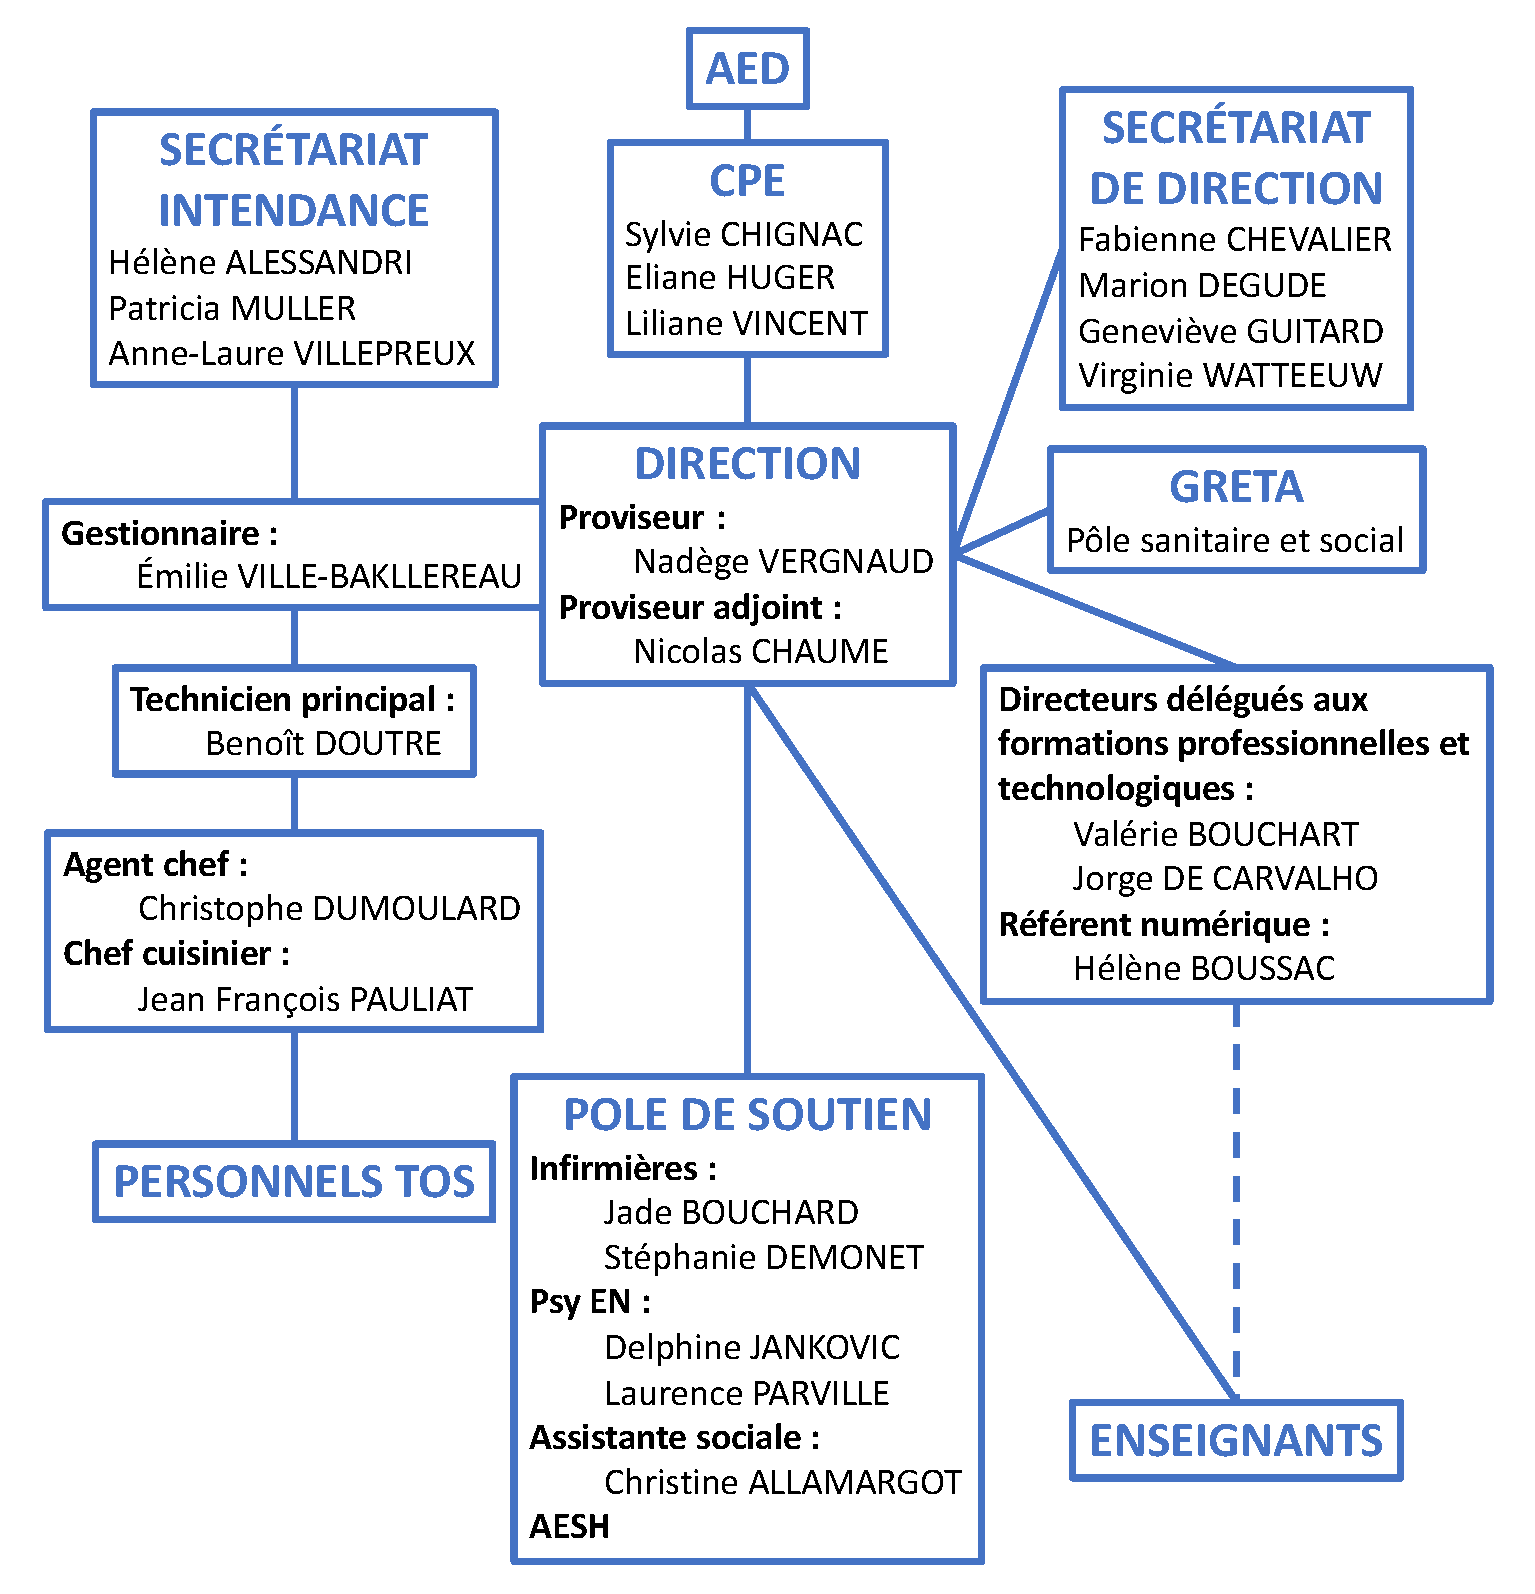
\includegraphics[width=\textwidth]{../../s3/rapport/organigramme.pdf}
\caption{Organigramme du lycée Suzanne Valadon.}
\label{fig:organigramme}
\end{figure}

\section{Emploi du temps}
\label{ann:edt}

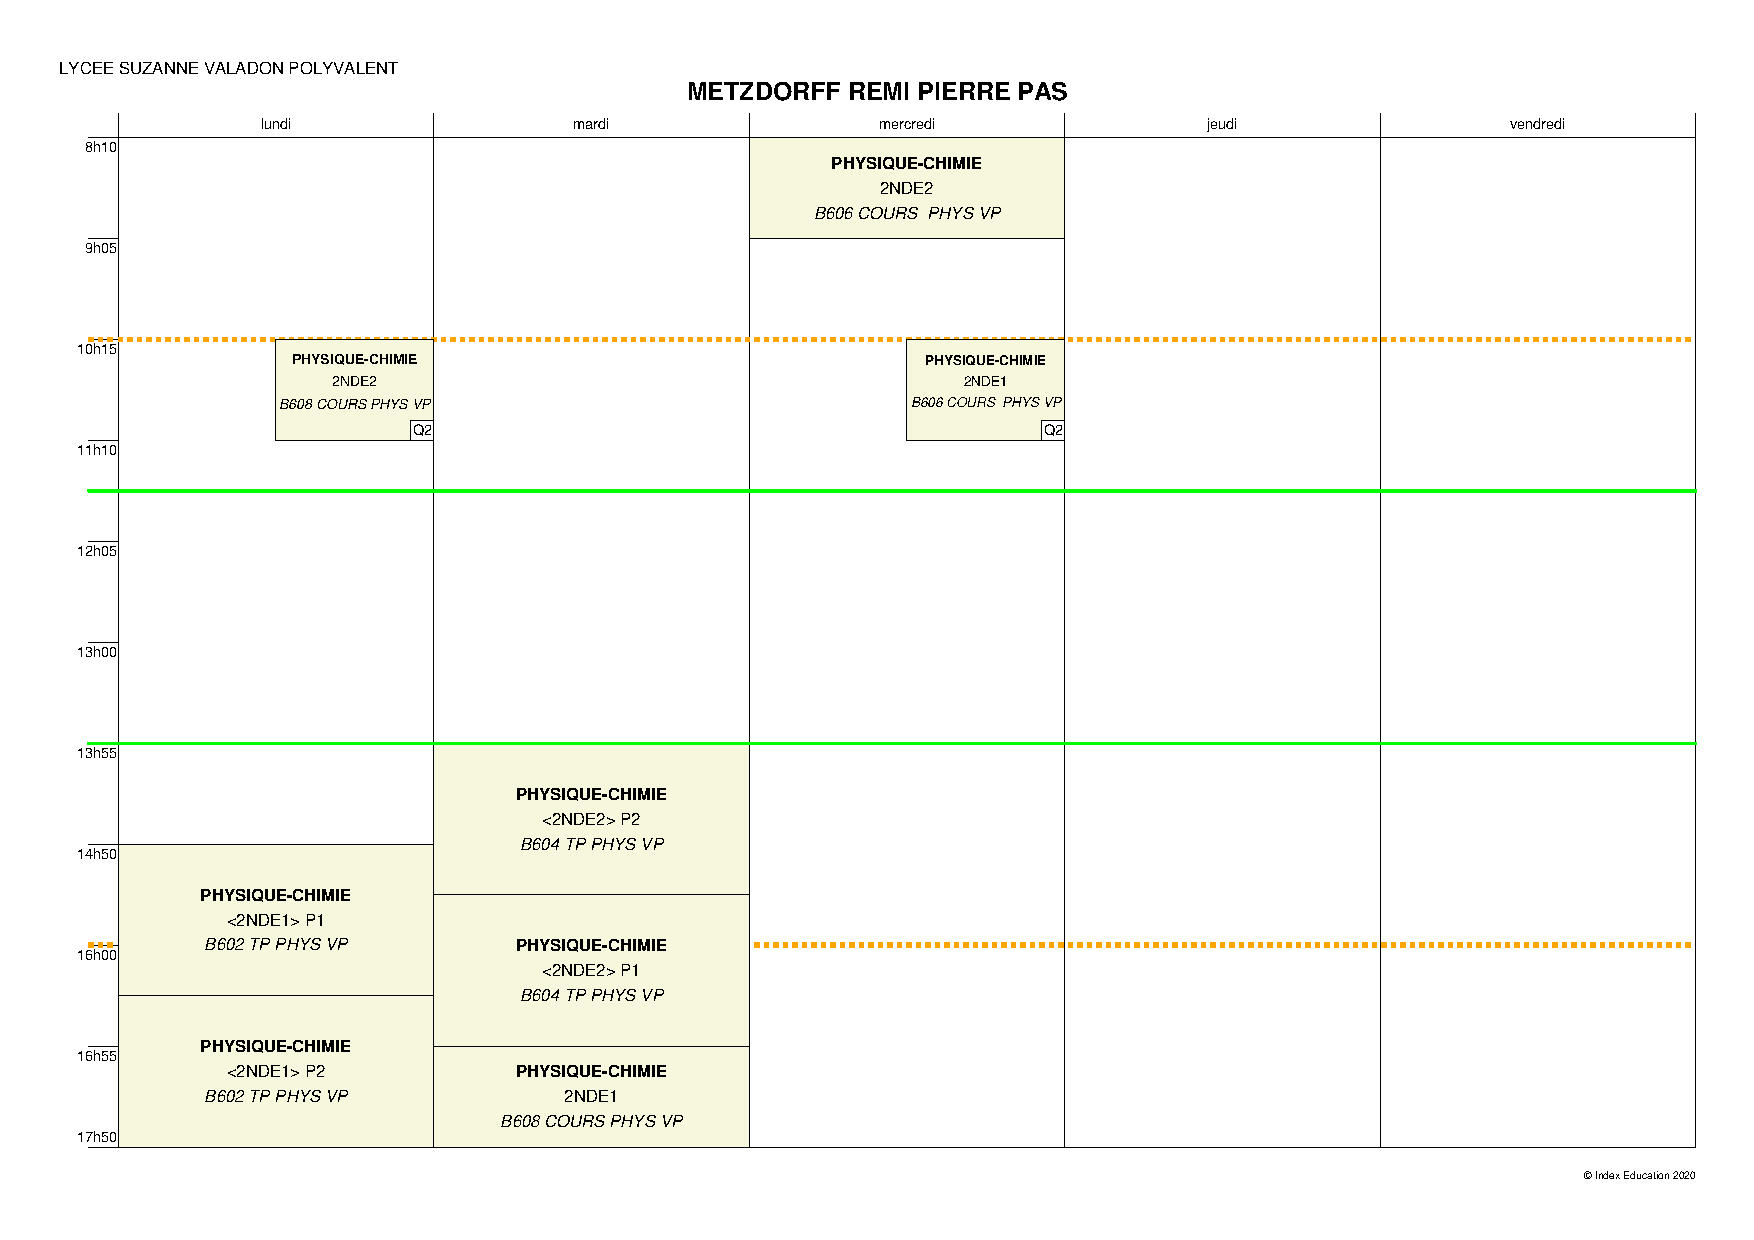
\includepdf[pages=-, landscape=true]{../../s3/rapport/edt_annuel.pdf}

\chapter{Sujet élève}

\section{Différenciation portant sur le document 2}
\label{ann:sujet_diff}

\begin{figure}[h]
\center
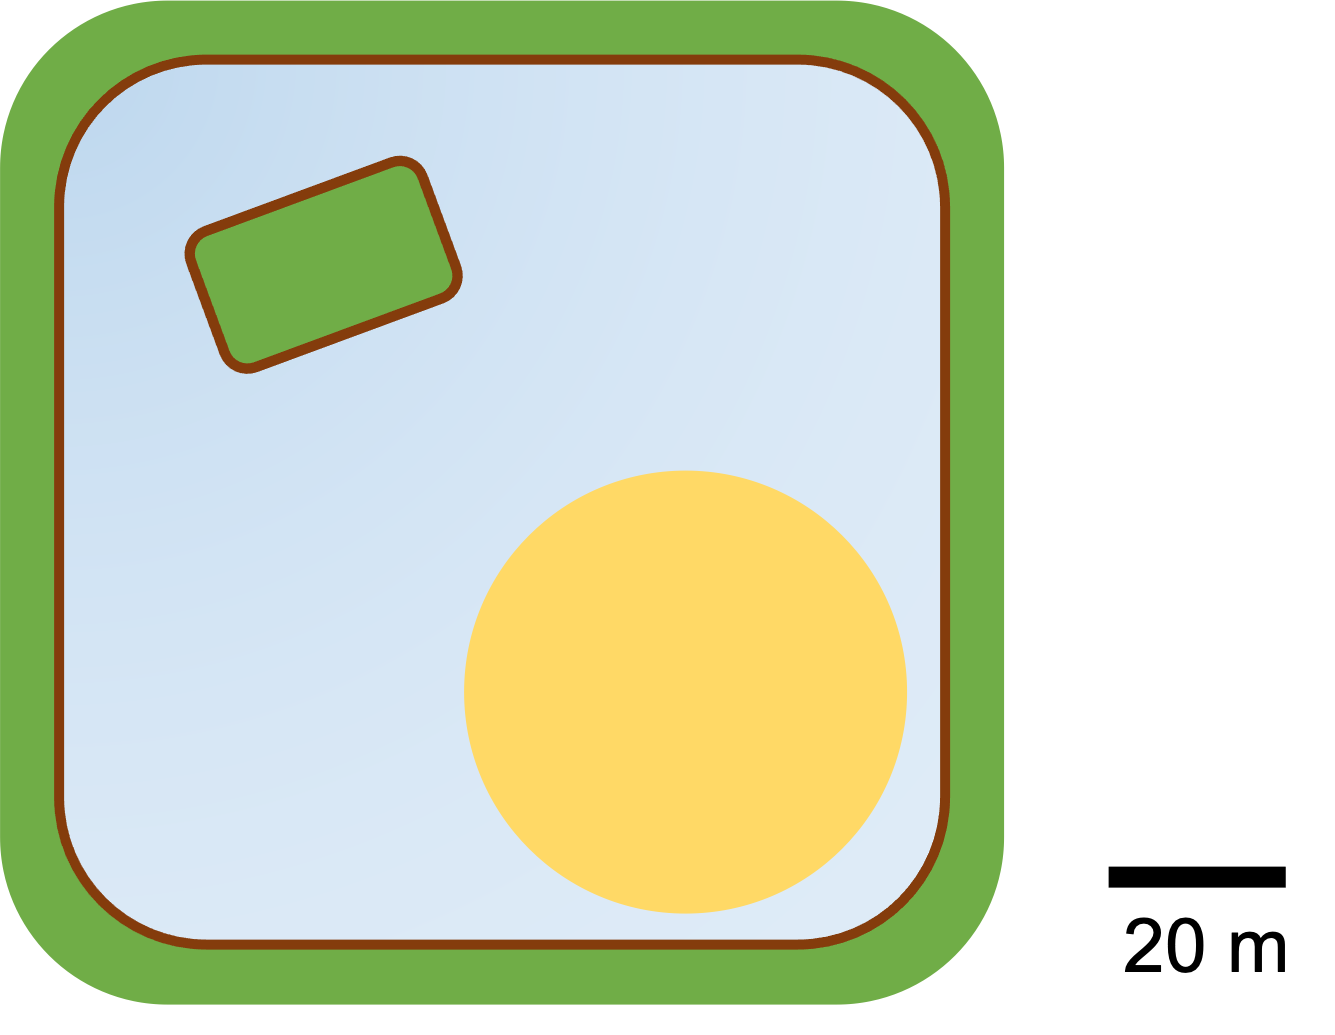
\includegraphics[scale=.3]{franklin_lake_diff1.png}
\hfill
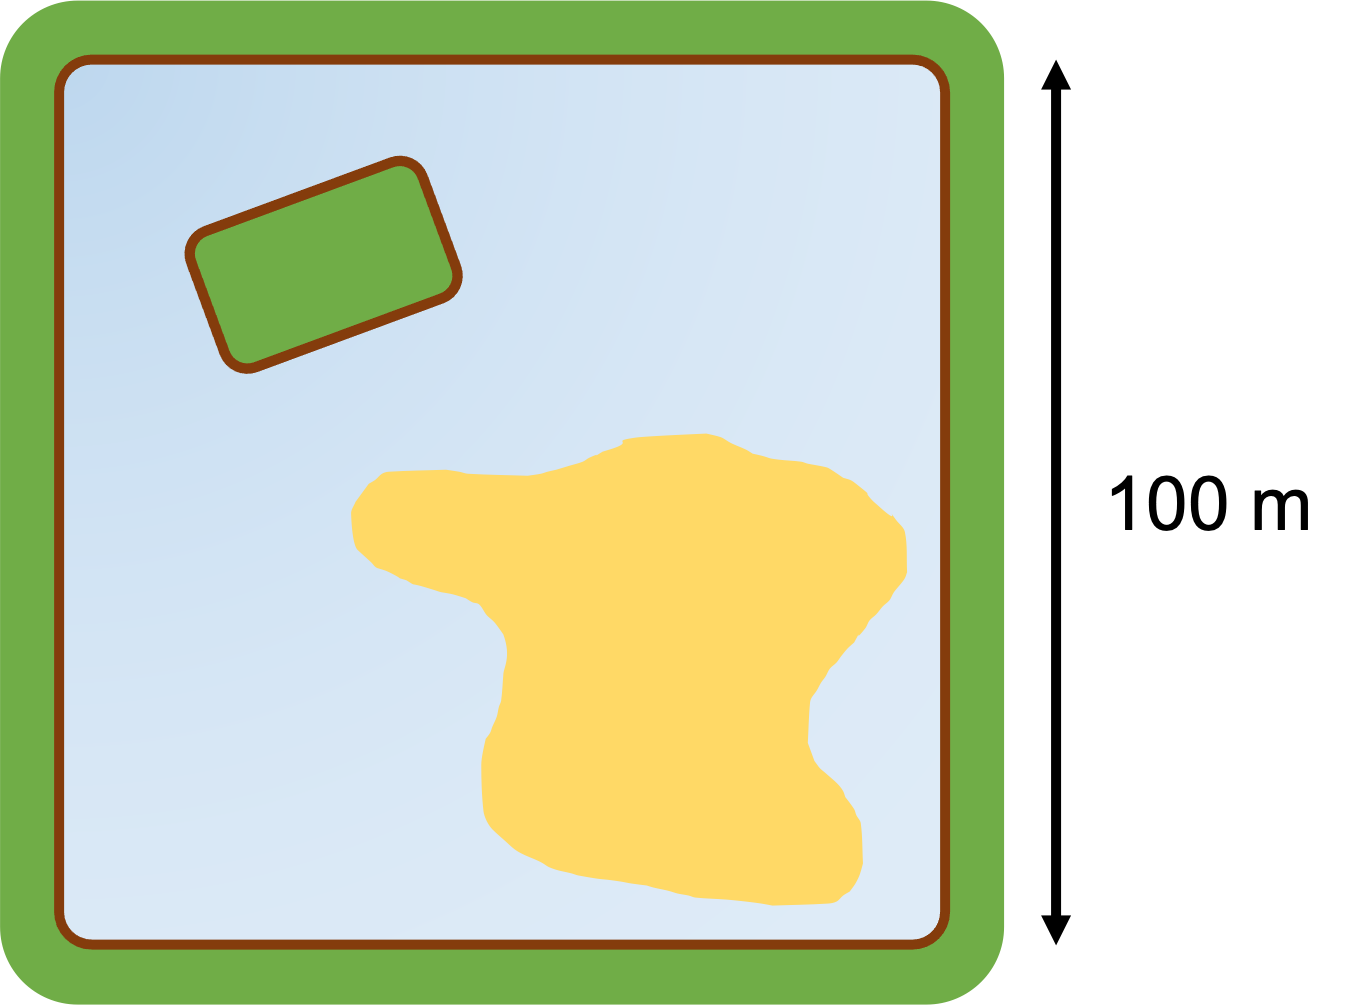
\includegraphics[scale=.3]{franklin_lake_diff2.png}

\caption{Deux schémas différents pour s'adapter à différents profils d'élèves.
À gauche : la version originale qui nécessite d'utiliser l'étalon de longueur pour déterminer la longueur d'un côté de l'étang ou le diamètre de la tache d'huile à l'aide d'un produit en croix.
À droite : la taille de l'étang est directement indiquée.
De plus, la forme indéterminée de la tache impose d'exploiter le texte (\og ce quart de l'étang \fg{}).
C'est donc la compétence \app{} qui sera mobilisée plutôt que la compétence \rea{}.
La forme de l'étang, plus proche d'un carré parfait, peut aussi éviter des interrogations quant aux coins arrondis qui nécessitent de faire une approximation supplémentaire pour le schéma de gauche.}

\end{figure}

\section{Sujet original}
\label{ann:sujet}

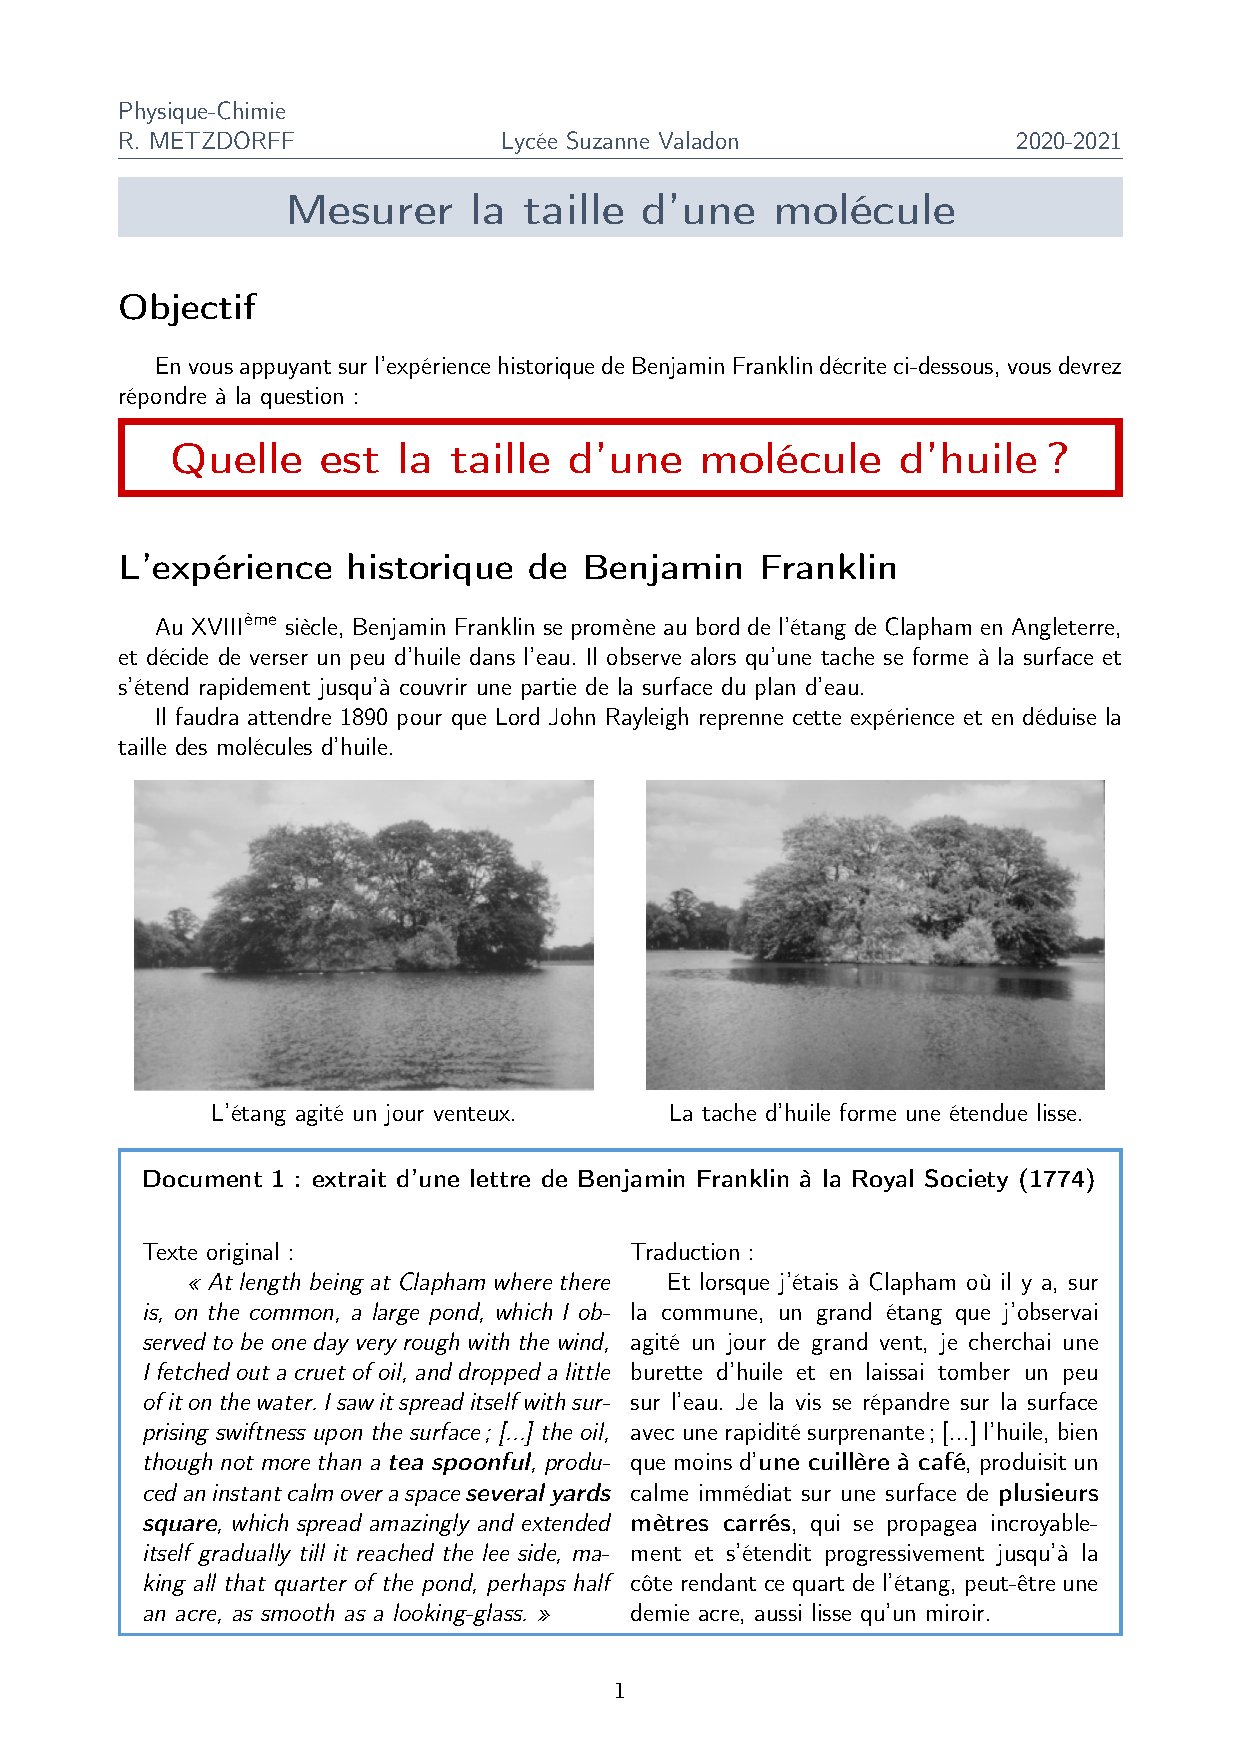
\includepdf[pages=-]{tp_franklin_v3.pdf}


\chapter{Proposition de correction}
\label{ann:corr}

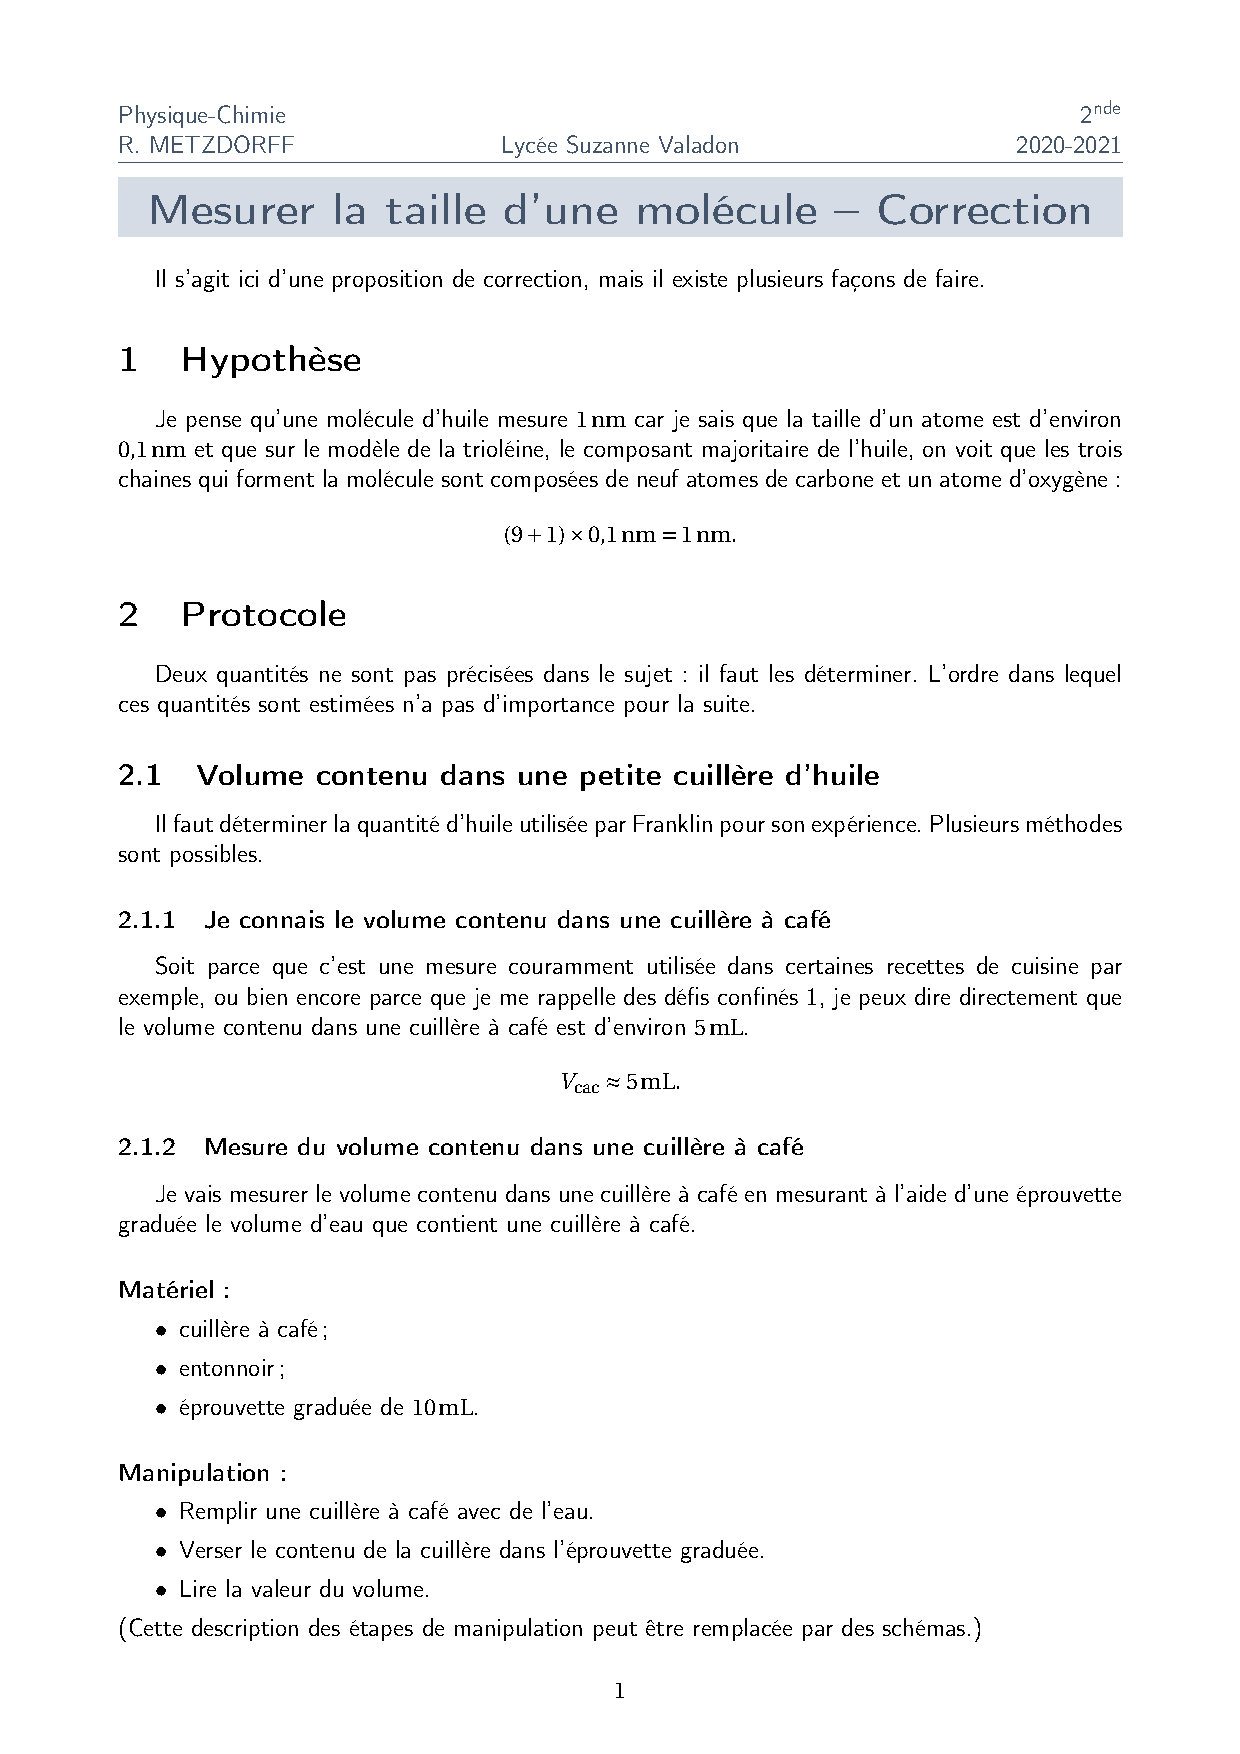
\includepdf[pages=-]{tp_franklin_corr.pdf}

\chapter{Aides}
\label{ann:aides}

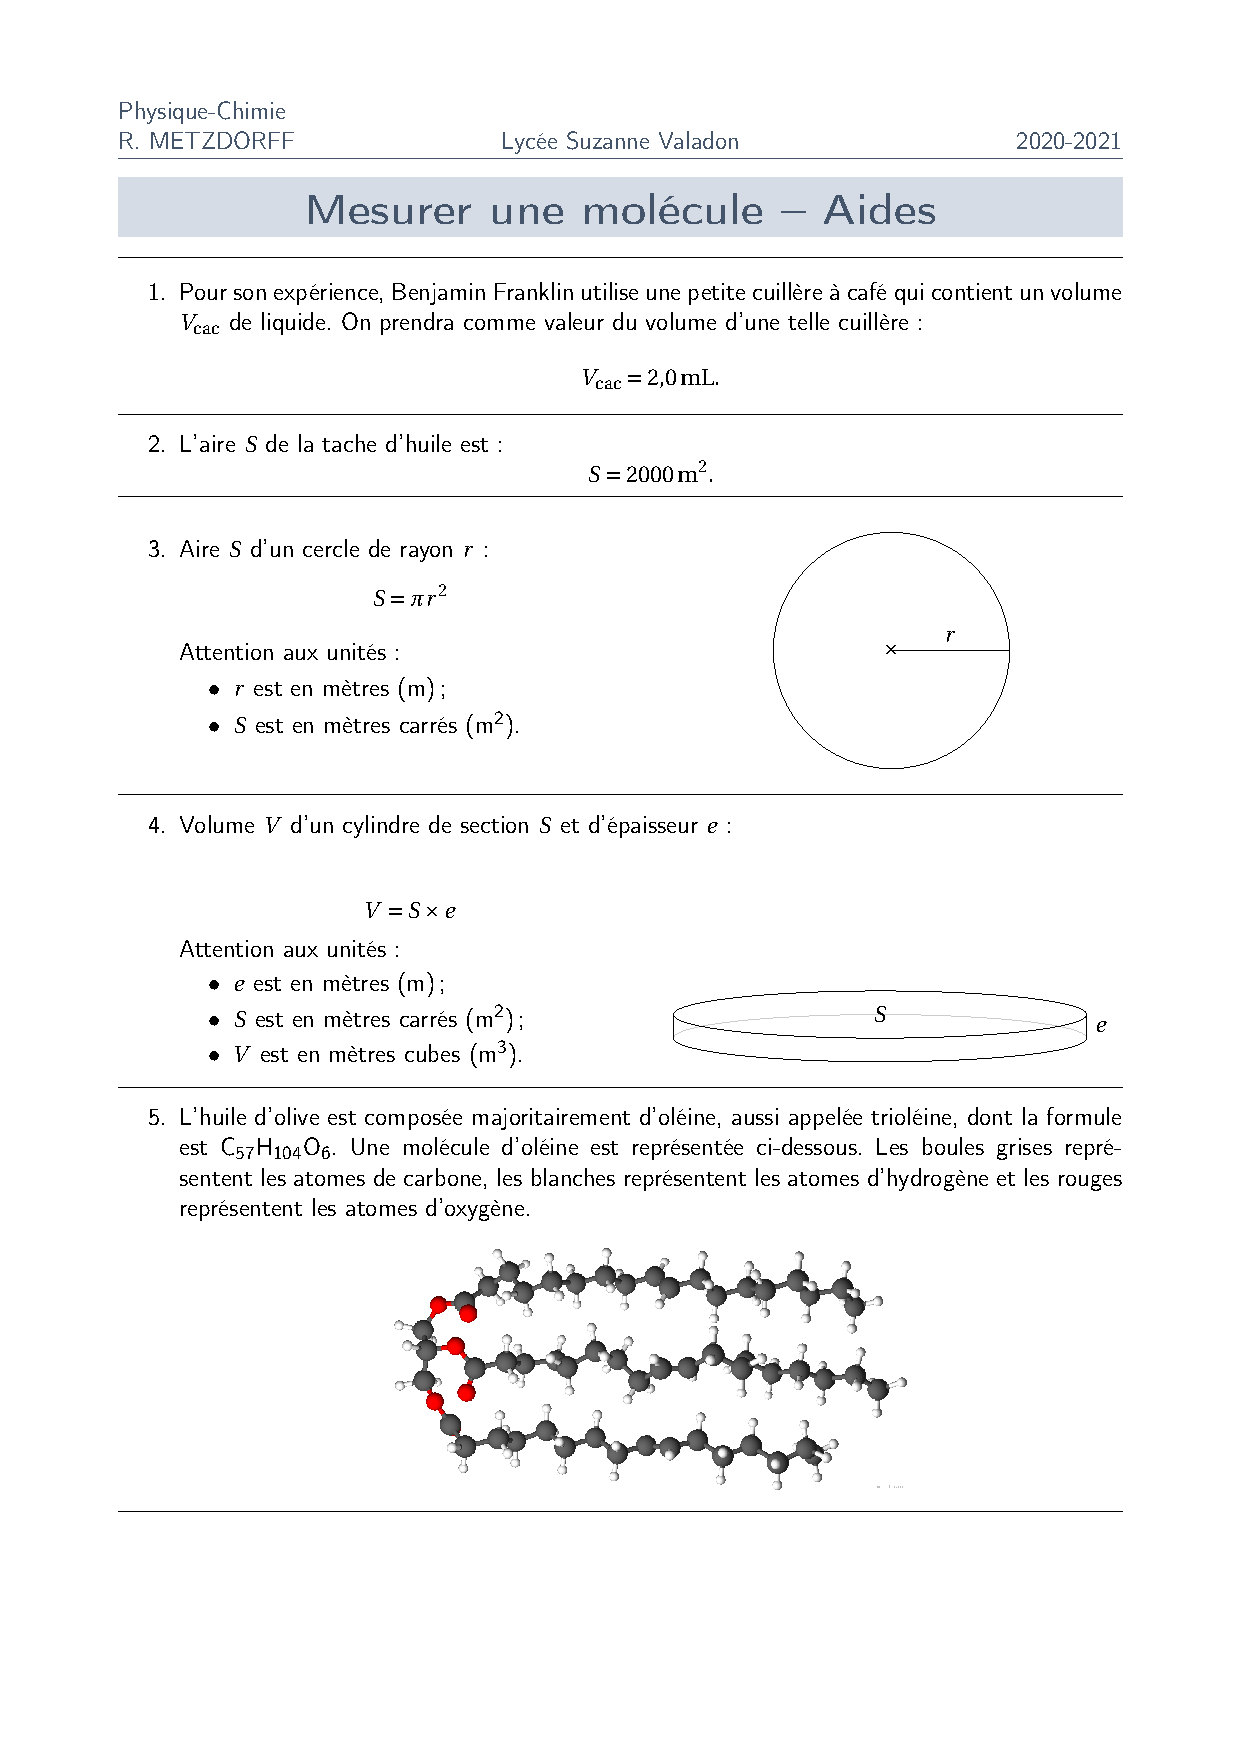
\includepdf[pages=-]{tp_franklin_aides.pdf}

\chapter{Fiche de suivi des élèves pendant la séance}
\label{ann:suivi}

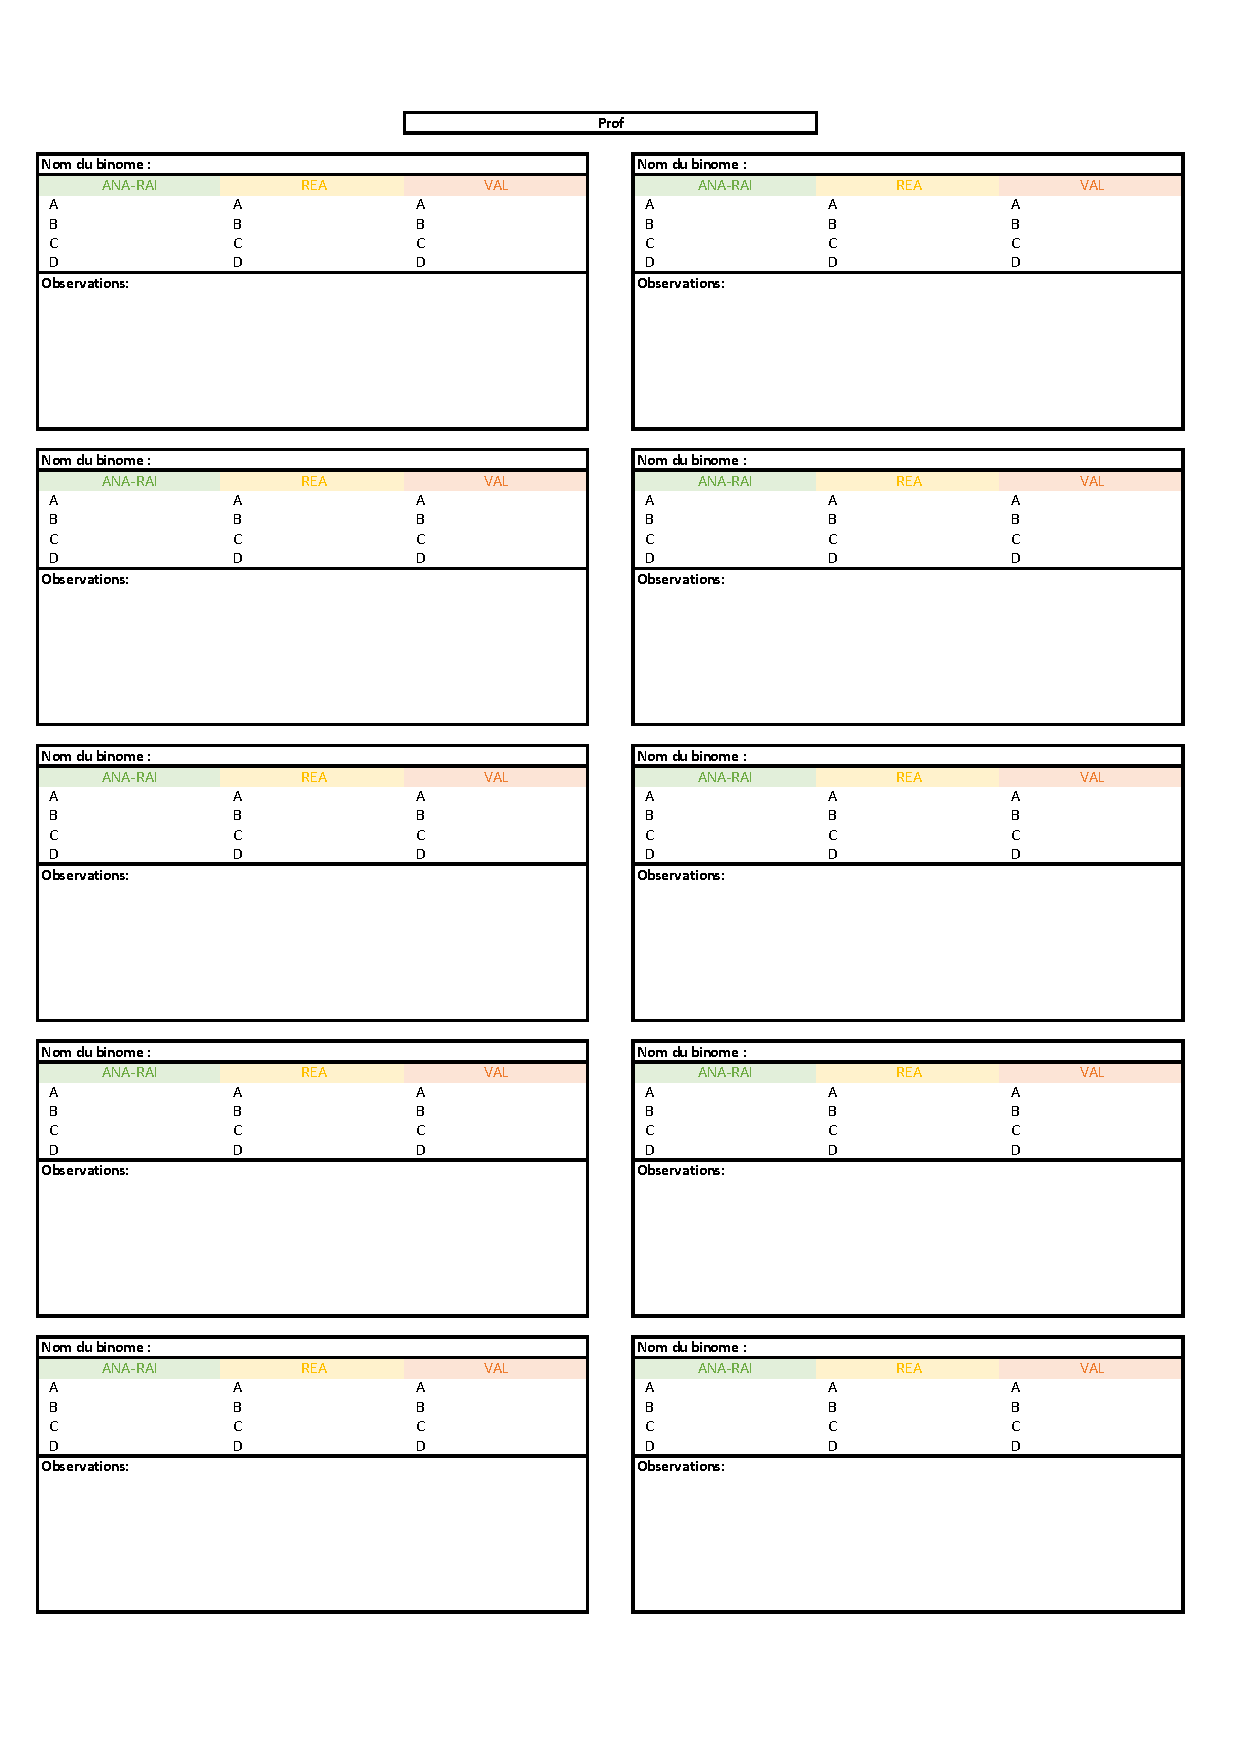
\includepdf[pages=-]{tp_franklin_prof_suivi-604.pdf}

\chapter{Fiche de suivi des élèves pendant la séance complétée}
\label{ann:suivi_comp}

\begin{landscape}

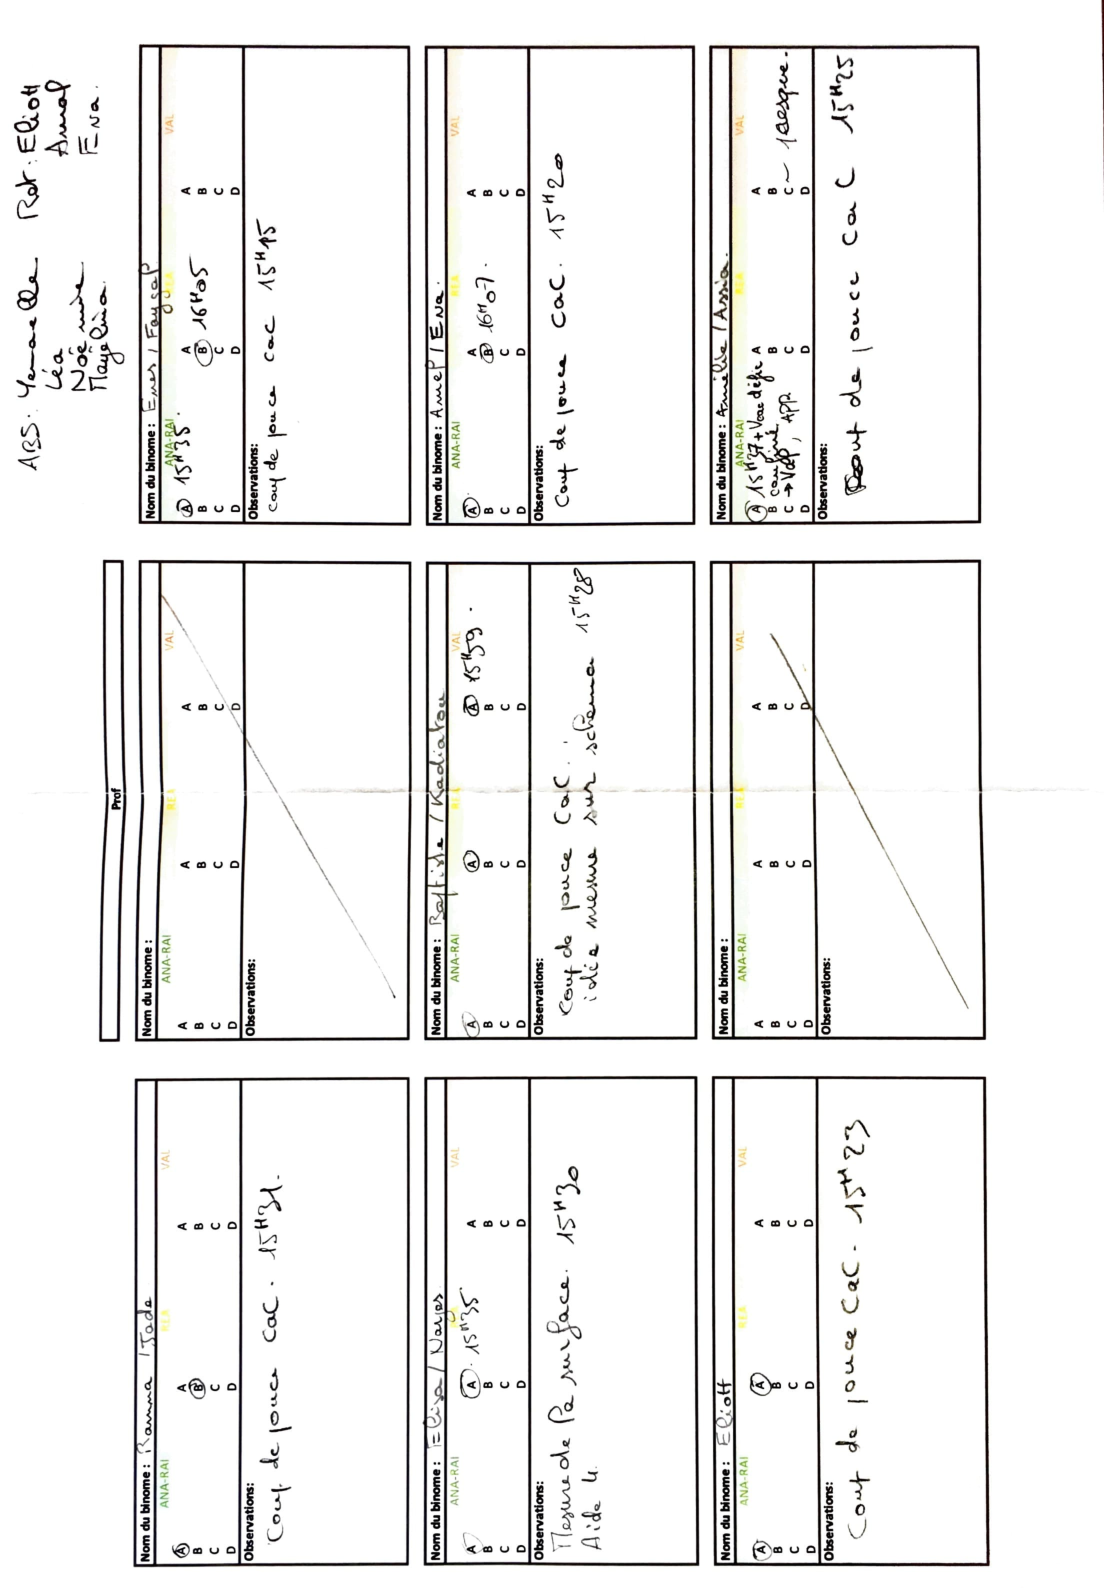
\includepdf[pages=-]{tp_franklin_prof_suivi.pdf}

\chapter{Évaluation de l'activité}
\label{ann:eval}
\vfill
\begin{table}[h]
\renewcommand\arraystretch{1.5}		% stretch table line height
\begin{center}
\begin{tabular}{|c|c|c|c|c|c|c|c|c|c|c|c|c|c|}
\hline
\textbf{Groupe} & \multicolumn{3}{c|}{\textbf{Séance}} & \multicolumn{4}{c|}{\textbf{Compte-rendu}} & \multicolumn{6}{c|}{\textbf{Total}} \\
\hline 
& \anarai & \rea & \val & \anarai & \rea &\val & \com & \app & \anarai & \rea & \val & \com & Note \\
\hline
& 5 & 5 & 3 & 1 & 3 & 2 & 1 & 0 & 6 & 8 & 5 & 1 & 20 \\
\hline\hline
\textbf{1} & A & B & & 1 & 2.5 & 0.5 & 1 & & 6 & 6.5 & 0.5 & 1 & 14 \\
\hline
\textbf{2} & A & A & & & 2.5 & 1.5 & 1 & & 5 & 7.5 & 1.5 & 1 & 15 \\
\hline
\textbf{3} & A & B & & 1 & 2 & 0.5 & 1 & & 6 & 6 & 0.5 & 1 & 13.5 \\
\hline
\textbf{4} & A & A & A & 1 & 2.5 & 1.5 & 1 & & 6 & 7.5 & 4.5 & 1 & 18 \\
\hline
\textbf{5} & A & A & & 0.5 & 0.5 & 0 & 1 & & 5.5 & 5.5 & 0 & 1 & 12 \\
\hline
\textbf{6} & A & B & & 1 & 1.5 & 0 & 1 & & 6 & 5.5 & 0 & 1 & 12.5  \\
\hline
\textbf{7} & A & B & C & 1 & 3 & 1 & 1 & & 6 & 7 & 2 & 1 & 16 \\
\hline
\end{tabular}
\end{center}
\caption{Bilan de l'évaluation de l'activité.}
\label{tab:eval}
\end{table}
\vfill
\end{landscape}

\chapter{Grille de notation pour l'oral}
\label{ann:oral}

\begin{figure}[htbp]
\center
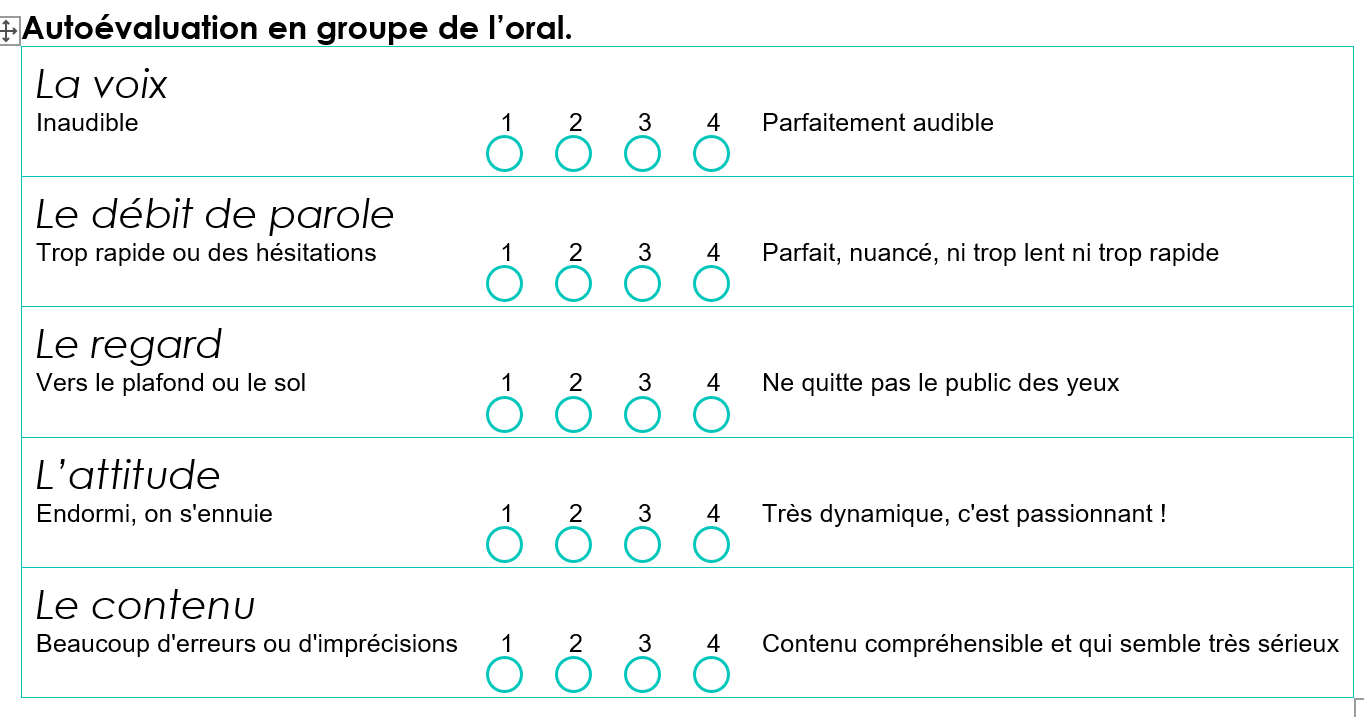
\includegraphics[width=\linewidth]{grille_notation_oral.png}
\end{figure}

\end{document}